\documentclass{report}

\usepackage[a4paper, total={6in, 8in}, margin=1in,footskip=0.25in]{geometry}
\usepackage{amsmath, amsthm, amssymb, booktabs, chemfig, graphicx, float, pgfplots, upgreek, siunitx, multirow, multicol, setspace}
% \usepackage[default]{sourcesanspro}
% \usepackage[T1]{fontenc}
\renewcommand{\familydefault}{\sfdefault}
\usepackage[hidelinks]{hyperref}
\usepackage{gensymb}
\newcommand{\perthousand}{‰}
\newcommand{\micro}{µ}
\usepackage[chemgreek=mhchem]{chemmacros}
\chemsetup[phases]{pos=sub}
\chemsetup[reactants]{concentration-unit=\moLar}
\chemsetup{
  formula = mhchem, % or mhchem
}

\DeclareSIUnit{\solub}{\unit[per-mode=symbol]{\gram\per\qty{100}{\gram}\,\ce{H2O}}}

\setlength{\parindent}{0pt}
\setlength{\parskip}{0.8em}

\pgfplotsset{compat=1.18}

\graphicspath{{../../Images/}}

\title{\Huge Year 12 Chemistry}
\author{L. Cheung}

\tolerance=1
\emergencystretch=\maxdimen
\hyphenpenalty=10000
\hbadness=10000

\begin{document}
	\maketitle
	\tableofcontents
	\DeclareSIUnit{\molar}{\mole\per\liter}
	\DeclareSIUnit{\enthalpy}{\kJ\per\mole}
	% !TEX root = ./chemistry.tex

\chapter{Module 5 \; Equilibrium and Acid Reactions}

\section{Le Chatelier's Principle} \label{29/10/2024-31/10/2024}
	"If a system at equilibrium is subject to a change in conditions, then the system will behave in such a way so as to partially counteract the imposed change"

	Haber process:

	\subsection{Effect of Concentration}
		\begin{equation}
			\ce{N2\gas{} + 3H2\gas{} <=> 2NH3\gas{} \quad \enthalpy{-92.5}}
		\end{equation}
		

	\subsection{Effect of Pressure}
	\subsection{Effect of Partial Pressure}
	\subsection{Effect of Volume}
		Decreasing the volume will increase the pressure. (Boyle's Law) This increases the collision rate between the reactants and favours the forward reaction.

	\subsection{Effect of Temperature}
		filler text
	
	\subsection{Summary}
		To use Le Chatelier's principle to predict the outcome of a change in conditions, you need to consider the following points.
		\begin{enumerate}
			\item What change is imposed?
			\item What is the opposite of the change?
			\item Which reaction direction is favoured - the forward or reverse?
			\item Does equilibrium shift to the left or right?
			\item What happens to the concentrations of each aqueous substance or gas?
		\end{enumerate}

	\begin{figure}[H]
		\centering
		\includegraphics{Le Chatelier's example problem}
	\end{figure}

	\textbf{D} When temperature decreases, the rates of both forward and backward reactions will decrease regardless of which way the endothermic or exothermic reaction goes. (A and B can be eliminated)

	This is because all the particles in the system lose kinetic energy, decreasing the rate of collisions hence, decreasing the rate of reaction.
	
	However, since there is a decrease in temperature the exothermic reaction will be favoured in order to counteract the change. In this case, the forward reaction being exothermic is affected less by the drop in temperature as shown in D.

\pagebreak
\section{Practical Investigation 2.3 - Effect of changes to concentration on equilibrium} \label{31/10/2024}

	Aim: To observe the effect of a change in concentration on a system at equilibrium

	\subsection{Materials}
		\begin{itemize}
			\item 2 mL of 0.1 molL$^{-1}$ iron(III) chloride solution
			\item 2 mL of 0.1 molL$^{-1}$ ammonium thiocyanate solution
			\item 1 mL of 0.1 molL$^{-1}$ calcium fluoride solution
			\item 20 mL distilled water
			\item 2x 10 mL measuring cylinders
			\item 25 mL measuring cylinder
			\item 4 test tubes
			\item Test-tube rack
			\item 4 small labels
			\item Disposable 1 mL droppers
			\item Waste bottle
			\item Digital camera
			\item Safety glasses
		\end{itemize}

	\subsection{Risk Assessment}
		\begin{table}[htbp]
			\centering
			\begin{tabular}{l|l}
				\hline
				Hazard & Precaution \\ \hline
				Chemicals may splash onto skin or eyes & Wear safety glasses and wash hands  \\
				Chemicals may harm aquatic life & Place in inorganic waste container \\
			\end{tabular}
		\end{table}

	\subsection{Method}
		\begin{enumerate}
			\item Pour 1 mL of iron(III) chloride solution into a 10 mL measuring cylinder.
			\item Pour 1 mL of ammonium thiocyanate into another 10 mL measuring cylinder.
			\item Pour both solutions into the 25 mL measuring cylinder.
			\item Add 18 mL of distilled water to the 25 mL measuring cylinder so that the total volume is 20 mL.
			\item Label four test tubes A, B, C and D.
			\item Pour equal volumes of the solution in the 25 mL measuring cylinder into each of the test tubes.
			\item Retain test tube A as the reference solution.
			\item Add 1 mL of iron(III) chloride to test tube B.
			\item Take a photo to record observations for test tube B relative to test tube A.
			\item Add 1 mL of ammonium thiocyanate to test tube C.
			\item Take a photo to record observations for test tube C relative to test tube A.
			\item Add 1 mL of calcium fluoride to test tube D. (Note: This reacts with the iron(III) ion so there is less iron(III) available to react with the thiocyanate ion.)
			\item Take a photo to record observations for test tube D relative to test tube A
		\end{enumerate}

	\subsection{Results}
		\begin{figure}[H]
			\centering
			\includegraphics{Practical Investigation 2.3 - Results.png}
			\caption{Test tubes A, B, C, D}
		\end{figure}

	\subsection{Discussion}
		\textbf{Explain each colour change in terms of collision theory.}

		The test tube B was darker in colour in comparison to test tube A. The increase in moles of reactants allows more successful collisions to occur, increasing the amount of product. The same principle applies to test tube C.

		Test tube D was lighter in colour compared to A, due to the calcium fluoride reacting with the iron (III) chloride 

	\subsection{Conclusion}
		\textbf{Use Le Chatelier's principle to explain what happened in test tubes B, C and D.}

		Test tube B was darker due to the increase in concentration of the reactant iron (III) chloride causes a shift of the equilibrium towards the products due Le Chatelier's principle
		
		Test tube C was darker due to the increase in concentration of the reactant ammonium thiocyanate causes a shift of the equilibrium towards the products due Le Chatelier's principle

		Test tube D was lighter because the calcium fluoride reacted with the iron (III) chloride, lowering the overall concentration of iron (III) chloride. This reduced the amount of reactants available, making the reverse reaction more favourable by Le Chatelier's principle.

\section{Calculating the Equilibrium Constant} \label{5/11/2024}
	The equilibrium constant can be used to predict the direction of chemical reactions

	$$K_{eq} = \frac{[products]}{[reactants]}$$
	For reaction:
	$$\ce{aA + bB <=> cC + dD}$$
	the equilibrium expression is:
	$$K_{eq}=\frac{[C]^{c}[D]^{d}}{[A]^a[B]^b}$$

	The concentration of each chemical species is raised to the power of the number of moles of that species indicated in the chemical equation. (Eg. there are $d$ moles of species $D$, hence in the equilibrium expression the concentration of species $D$ is raised to the power of $d$, written as $[D]^d$)

	\begin{itemize}
		\item The value for the equilibrium constant only takes into account the concentration of substances where the concentration can vary
		\item Solutions and gases can vary in concentration or partial pressure hence are included in $K_{eq}$
		\item Solids and pure liquids are NOT included eg. $\ce{H_2O}$ isn't required when calculating
	\end{itemize}

	\subsection{Reaction Quotient ($Q$)}
		$$Q=\frac{[C]^{c}[D]^{d}}{[A]^a[B]^b}$$
		Has the same formula as $K_{eq}$, however applies to any stage of a reaction
		
	\subsection{Equilibrium Constant}
		\begin{itemize}
			\item Comparing $Q$ to $K_{eq}$ predicts which way the equilibrium will shift
			\item $K_{eq}$ is where the equilibrium lies
			\item A large $K_{eq}$ means that there are more products than reactants; ie. equilibrium lies towards completion
			\item If $K_{eq}$ is close to one, both reactants and products are plentiful at equilibrium
		\end{itemize}
		\textbf{Example} Let $Q=2.1$, $K_{eq}=0.315$, $\therefore$ products$>$reactants.

	\subsection{Calculating the equilibrium expression}
		Consider the reaction between hydrogen and iodine producing hydrogen iodide:
		$$\ce{H_{2}\gas{} + I_{2}\gas{} <=> 2HI\gas}$$

\section{ICE Tables} \label{6/11/2024}
	\begin{table}[htbp]
		\centering
		\begin{tabular}{|l|l|l|l|}
			\hline
			 & [A] & [B] & [C] \\ \hline
			Initial concentration &  &  &  \\
			Change in concentration &  &  &  \\
			Equilibrium concentration &  &  &  \\ \hline
		\end{tabular}
	\end{table}

	$$\Delta c = c_{eq}- c_{u}$$

	Eg. $\ce{A + B <=> C + D}$

	\begin{table}[htbp]
		\centering
		\begin{tabular}{lllll}
			\hline
			 & [A] & [B] & [C] & [D]  \\ \hline
			Initial concentration 		& 0.6 & 0.6 & 0 & 0 \\
			Change in concentration 	& -0.5 & -0.5 & +0.5 & +0.5 \\
			Equilibrium concentration 	& 0.1 & 0.1 & 0.5 & 0.5 \\ \hline
		\end{tabular}
	\end{table}

	Eg. $\ce{2X \gas{} <=> 3Y \gas{} + 4Z \gas{}}$

	A sample consisting of 0.500 mol of X is placed into a system with a volume of 0.750 litres. \\
	At equilibrium, the amount of sample X is known to be 0.350 mol.

	\begin{table}[htbp]
		\centering
		\begin{tabular}{cccc}
			\hline
			 & X & Y & Z \\ \hline
			I 		& 0.5 & 0 & 0 \\
			C 		&  &  & \\
			E 		& 0.35 &  &  \\ \hline
		\end{tabular}
	\end{table}

	\begin{table}[htbp]
		\centering
		\begin{tabular}{cccc}
			\hline
			 	& X & Y & Z \\ \hline
			I 		& 0.5 & 0 & 0 \\
			C 		& -0.15 & -0.225 & +0.3 \\
			E 		& 0.35 & 0.225 & 0.3 \\ \hline
		\end{tabular}
	\end{table}

	\begin{align*}
		[X] &= \frac{0.35}{0.75} = 0.467 \\
		[Y] &= \frac{0.225}{0.75} = 0.3 \\
		[Z] &= \frac{0.3}{0.75} = 0.4
	\end{align*}
	
\section{Effect of Temperature on $K_{eq}$} \label{8/11/2024}
	Although other factors may affect equilibrium, $K_{eq}$ is only affected by temperature.
	Changing concentration, pressure, or volume will change the concentrations and therefore adjust the reaction point, however the reaction will still equalise to achieve the same $K_{eq}$

	\begin{itemize}
		\item For a particular reaction, $K_{eq}$ is constant at a given temperature
		\item Temperature changes the ratio of products and reactants, hence changing $K_{eq}$
		\item For $\ce{N2O2 \gas{} <=> 2NO2 \gas{}}$, temperature increases the $K_{eq}$ value and favours the formation of products. The forward reaction is endothermic
	\end{itemize}

	\subsection{Example Question}
		Nitric oxide gas ($\ce{NO}$) can be produced from the direct combination of nitrogen gas and oxygen gas in a reversible reaction.
		\begin{enumerate}
			\item \textbf{Write a balanced chemical equation for this reaction (1 mark)}
				\subitem $\ce{N2 \gas{} + O2 \gas{} <=> 2NO \gas{}}$
			\item \textbf{Explain, using collision theory, how an increase in temperature would affect the value for $K_{eq}$ for this system. Refer to the diagram in your answer.}
				\subitem An increase in temperature would favour the forward reaction, hence $K_{eq}$ will increase. More energy allows more collisions to occur
		\end{enumerate}
	
		\begin{align*}
			K_{eq} &= \frac{[p_1][p_2]}{[r_1][r_2]} \\
			1 &= \frac{[1][1]}{[1][1]} \\
		\end{align*}
		\text{\centering If $p_2$ decreases to $[0.5]$, favouring the forward reaction}
		\begin{align*}
			&= \frac{[1.15][0.65]}{[0.85][0.85]} \\
			&=K_{eq}
		\end{align*}

\section{Use of $K_{eq}$ for the Dissociation of Ionic Solutions} \label{12/11/2024}
	Different ionic compounds have different solubilities

	Example reaction

	$$\ce{AgNO3 \aq{} + NaCl \aq{} -> AgCl \sld{} + NaNO3 \aq}$$

	Complete ionic equation: $\ce{Ag+ + NO3-}$
	
	\section{Beer Lambert Law} \label{14/11/2024}
	\begin{align*}
		\text{Absorbance} &= \text{Molar absorbility} \times \text{Path length} \times \text{Concentration} \\
		A &= \epsilon lc
	\end{align*}
	\begin{itemize}
		\item Absorbance has a direct relationship to concentration
		\item Greater concentration, greater absorbance
	\end{itemize}
	
\section{Practical Investigation 3.2}
	Aim: To use colourimetry to determine the equilibrium constant for the reaction of iron(III) ions with thiocyanate ions to form the iron(III) thiocyanate ion

	\subsection{Materials}
		\begin{itemize}
			\item 200 mL 0.2 \unit{\moLar} $\ce{Fe(NO3)3}$
			\item 100 mL 0.002 \unit{\moLar} $\ce{KSCN}$
			\item 500 mL 0.5 \unit{\moLar} $\ce{HNO3}$
			\item 60 mL 0.002 \unit{\moLar} $\ce{Fe(NO3)3}$
			\item 150 mL distilled water
			\item 6 * 100 mL volumetric flasks
			\item 5 * 150 mL beakers
			\item 2 * 100 mL beakers
			\item 1 * 25 mL bulb pipette
			\item 2 * 10 mL graduated pipettes
			\item 1 * 10 mL bulb pipette
			\item 2 pipette bulbs
			\item 1 disposable pipette
			\item Waste bottle
			\item 14 small labels
			\item 1 colourimeter and set of cuvettes
			\item Safety glasses
		\end{itemize}

	\subsection{Risk Assessment}
		\begin{table}[htbp]
			\centering
			\begin{tabular}{ll}
				\hline
				Hazard & Precaution \\ \hline
				Breaking glassware & Keep glassware on inside of table, do not run with glassware \\
				Spillage of solutions & Handle with caution, clean any spills immediately \\
				Splashing of solution into eyes & Wear safety goggles \\ \hline
			\end{tabular}
		\end{table}
	
	\subsection{Method}
	\begin{enumerate}
		\item Label the six volumetric flasks A-F.
		\item Use a 25 mL bulb pipette to transfer 25.00 mL of the 0.200 \unit{\moLar} $\ce{Fe(NO3)}$\item 3 to flask A.
		\item Use a graduated 10 mL pipette to transfer 1.00 mL of the 0.002 \unit{\moLar} \item $\ce{KSCN}$ to flask A.
		\item Add HNO3 to make a final volume of 100.00 mL.
		\item Make solutions with known concentration by pushing equilibrium as far as possible to the products. $\ce{HNO3}$ can be used to reduce the concentration of $\ce{H3O}$
		\item Rinse the cuvette with distilled water.
		\item $\frac{3}{4}$ fill the cuvette with distilled water and wipe the clear sides. 
		\item Turn on the colourimeter and turn the light to blue or 470 nm.
		\item Use the cuvette with distilled water to calibrate the colourimeter. Note: Orientate the cuvette correctly in the colourimeter so that the light passes through the clear sides of the cuvette.
		\item Rinse, a 100 mL beaker with standard solution A - it is easier to pour the solution into the cuvette using a beaker than using a volumetric flask.
		\item Rinse, then $\frac{3}{4}$ fill the cuvette with standard solution A and measure the absorbance with the colourimeter.
		\item Repeat steps 10 and 11 for the other standard solutions (B-F)
	\end{enumerate}

\section{Solution Equilibria - Dissolution of Ionic Compounds} \label{19/11/2024}
	\subsection{Factors influencing solubility}
		\begin{itemize}
			\item Activation energy required to break lattice
				\begin{itemize}
					\item Strength of ionic bonding
					\item Size of ions
					\item Charge of ions
				\end{itemize}
			\item As temperature increases, generally solubility increases
		\end{itemize}

	% !TEX root = ./chemistry.tex

\chapter{Module 6 \hspace{0.5em} Acid and Base Reactions} \label{12/12/2024}

	\section{Introduction to Acid and Bases}
	
		\textbf{General Properties of Acids}
		
			\begin{itemize}
				\item Sour taste
				\item Low pH
				\item Turn blue litmus paper red
				\item Corrosive
			\end{itemize}

		\textbf{General Properties of Bases}
			
			\begin{itemize}
				\item Bitter taste (eg. caffeine)
				\item High pH
				\item Turn red litmus paper blue
				\item Corrosive and caustic
			\end{itemize}

	\section{Indicators}
	
		Indicators are substances added to solutions to show their pH. They show the concentration of hydrogen ions in a solution through a colour change.

		Most indicators are \textbf{weak acids or bases} meaning they exist in equilibrium.acids or

		\begin{center}
			\ce{HIn <=> H+ + In-}, where \ce{In} stands for indicator
		\end{center}

		Eg. Added to an acidic solution:
		\begin{enumerate}
			\item Equilibrium is disturbed by the increase of \ce{H+} ions
			\item Equilibrium therefore shifts left to decrease this concentration (LCP)
			\item As a result, the concentration of \ce{HIn} Increases, therefore changing the colour
		\end{enumerate}

		Indicators are more useful in clear, colourless solutions that make it easier to identify the equivalence point.

		\textbf{Example Question}

			\begin{figure}[H]
				\centering
				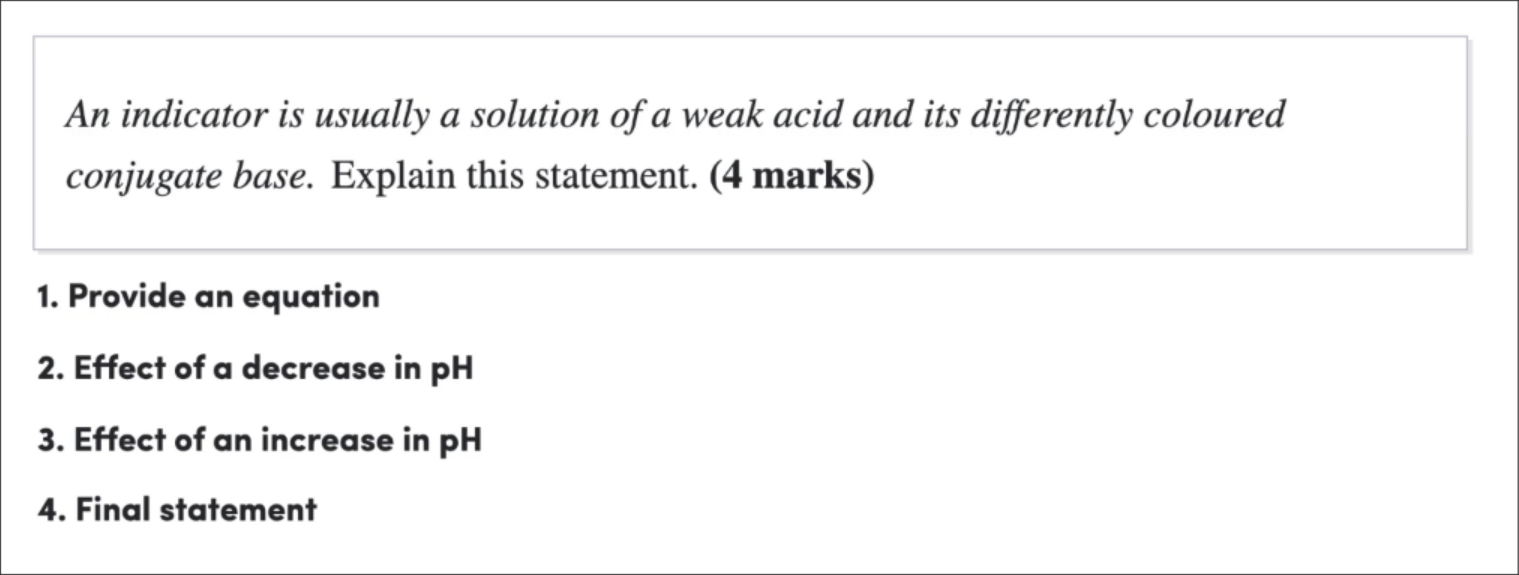
\includegraphics[width=15cm]{indicators_question.png}
			\end{figure}

		\subsection{Common Indicators}
		
			\begin{table}[H]
				\centering
				\setstretch{1.5}
				\begin{tabular}{p{4cm}| p{5cm} | p{5cm}}
					Indicator	& pH Range	& Colour (increasing pH) \\ \hline
					Methyl orange	& 3.1 - 4.4	& Red - Orange - Yellow \\
					Liquid litmus	& 4.5 - 8.3	& Red - Purple - Blue \\
					Bromothymol blue& 6.0 - 7.6	& Yellow - Green - Blue \\
					Phenolphthalein	& 8.3 - 10.0	& Colourless - Pale pink - Bright pink \\
					Universal indicator & All pH	& Red - Violet
				\end{tabular}
			\end{table}

\section{Practical Investigation 5.1 - Preparing and using natural indicators}

	Aim: To prepare and test natural indicators on a range of substances to determine their acidity or alkalinity

	\subsection{Materials}
		\begin{itemize}
			\item Plant material that acts as an indicator (Eg. red cabbage, blueberries, turmeric, petals from violets, geranium, petunias)
			\item Approx. 5mL of:
			\begin{itemize}
				\item \qty{0.1}{\moLar} NaOH
				\item \qty{0.1}{\moLar} HCl
				\item white vinegar
				\item household ammonia
				\item lemon juice
				\item lemonade
				\item bicarbonate of soda
				\item washing powder
				\item antacid tablet
				\item salt water
			\end{itemize}
			\item Distilled water
			\item \qty{500}{mL} beaker
			\item \qty{100}{mL} beakers
			\item Test tubes
			\item Test-tube rack
			\item \qty{10}{mL} measuring cylinder
			\item Knife
			\item Cutting board
			\item Mortar and pestle
			\item Kettle (for warm water)
			\item Hotplate
			\item Spatula
			\item Droppers
			\item Stirring rod
			\item Strainer or filter paper and funnel
			\item Safety glasses
		\end{itemize}

	\subsection{Risk Assessment}
		\begin{table}[H]
			\centering
			\begin{tabular}{ll}
				\hline
				Hazard & Precaution \\ \hline
				Acids are corrosive, irritate eyes & Handle with caution \\
				Bases are caustic, irritate eyes & Handle with caution \\ \hline
				Ammonia is caustic & Use in well ventilated areas \\ \hline
			\end{tabular}
		\end{table}
	
	\subsection{Method}
		\begin{enumerate}
			\item For the red cabbage: Finely shred two leaves of cabbage, place in 500 mL beaker and just cover with distilled water (about 200 mL). Slowly boil the cabbage leaves until the water turns a dark reddish-purple and the leaves lose most of their colour.
			\item Allow to cool and pour the liquid off into a clean 100 mL beaker. This is the red cabbage indicator. Note: If the colour of the solution is pale, further boiling may be necessary to concentrate the solution.
			\item For other plant material: Cut the material into small pieces and place in a mortar and pestle. Grind the material to a paste, add 5-10 mL of warm water and stir.
			\item Strain the solution into a beaker to remove any solids.
			\item Place 2 mL of each of NaOH and HCl into clean separate test tubes. Add a few drops of one indicator to each test tube until a definite colour is observed. Record the indicator and its colour in your results table.
			\item Repeat step 5 with other indicators and record your results in the table. 
			\item Repeat steps 5 and 6 with other substances. Classify the substances as acidic, basic or neutral.
			\item Place 2 mL of HCl in a clean test tube. Choose an indicator that produced a good colour difference between acid and base and add a few drops to the test tube.
			\item Add NaOH a few drops at a time to the HCl test tube until the colour no longer changes. Record any colour changes that occur during the addition of NaOH.
			\item To the test tube from step 9 add HCl a few drops at a time until the colour no longer changes. Record any colour changes.
		\end{enumerate}

	\subsection{Results}

	\subsection{Discussion}
		\begin{enumerate}
			\item \textbf{Identify which indicators would be most effective in identifying acidic, basic and neutral solutions. Provide 
			a reason for your choice.}
			Acid
			Neutral
			Basic
			\item \textbf{Which indicators, if any, were not effective in distinguishing between acidic, basic and neutral solutions? 
			Suggest possible reasons for this.}
			\subitem The beetroot and blue tea indicators were not as effective compared to the universal indicator. For unknown solutions, universal indicator allows identification of the pH. Blue tea has a lower concentration of anthocyanin compared to the beetroot solution, therefore was less effective as an indicator.
			\item \textbf{Using your results, justify whether or not indicator colour change is a reversible reaction.}
			\subitem It is a reversible reaction
		\end{enumerate}
	
	\subsection{Conclusion}
	\begin{enumerate}
		\item \textbf{Explain why indicators give a range of colours in different acid and alkaline solutions.}
	\end{enumerate}

\section{History of Acid-Base Models} \label{10/02/2025}
	\textbf{Lavoisier - Acids contain oxygen}
	\begin{itemize}
		\item Correct for some acids, eg. $\ce{H2SO4}$
		\item However doesn't apply to all acids, eg. $\ce{HCl}$ doesn't have oxygen
	\end{itemize}

	\textbf{Davy - Acids contain displaceable hydrogen}
	\begin{itemize}
		\item Considered reactions with metals and acid
		\item $\ce{H2}$ gas produced as metal displaces hydrogen in acid
		\item $\ce{H2(g) + 2HCl(aq) -> H2(g) + MgCl2(aq)}$
	\end{itemize}

	\textbf{Arrhenius - Acids ionise in water to form H+ ions}
	\begin{itemize}
		\item $\ce{HA(aq) -> H+(aq) + A-(aq)}$
		\item $\ce{XOH(aq) -> X+(aq) + OH-(aq)}$
		\item Couldn't explain why ammonia was a base
		\item Nature and role of the solvent was not considered
		\item All salts produced by reactions of an acid and base should be neutral, but acetic acid and sodium hydroxide results in a basic solution
	\end{itemize}

\section{Ammonia Dilemma} \label{12/02/2025} TODO:
	Ammonia ionises in water and produces $\ce{OH-}$ ions, and is therefore classified as an Arrhenius base. However, considering the following reaction:

	$$\ce{NH3(g) + HCl(g) -> NH4Cl(s)}$$

	The above reaction is an acid ($\ce{HCl}$) base (\ce{NH3}) reaction, however it doesn't form water.

	\subsection{Bronsted-Lowry Model}
 		Acids are proton donors, bases are proton acceptors
		\bgroup
			\centering
			\ce{HCl(aq) + H2O(l) -> H3O+(aq) + Cl-(aq)}
		\egroup

		In the above reaction, \ce{HCl} accepts a proton from \ce{H2O}, $\therefore$ \ce{HCl} = acid, \ce{H2O} = base

		\bgroup
			\centering
			\ce{NH3(aq) + H2O(l) -> NH4+(aq) + OH-(aq)}
		\egroup

		Water is \textbf{amphiprotic}, ie. can act as an acid or a base.

		\bgroup
			\centering
			\ce{2H2O <=> H3O+ + OH-}
		\egroup

		Limitations:
		\begin{itemize}
			\item Requires a solvent and doesn't explain for non-aqueous solutions
			\item Cannot explain for acidic oxides, eg. \ce{CaO(s) + SO3(g) -> CaSO4(s)}
			\item \ce{BF3}, \ce{AlCl3} act as acids, however have no \ce{H+} to donate.
		\end{itemize}

	\subsection{Lewis Model}
		Acid is an electron pair acceptor, base is an electron pair donator
		
		Explains the \ce{BF3 + NH3} reaction:

		Boron accepts a pair of electrons from the nitrogen in ammonia. Although no proton is transferred, it is still an acid-base reaction

\section{Practical Investigation 5.2 - Measuring the enthalpy of neutralisation} \label{13/02/2025}
	\textbf{Aim:} To determine the enthalpy of neutralisation and the effect of the state of the reactants

	\subsection{Materials}
		\begin{itemize}
			\item 4g NaOH
			\item 100mL 1.0 molL$^{-1}$ HCl
			\item 50mL 2.0 molL$^{-1}$ HCl
			\item 50mL 2.0 molL$^{-1}$ NaOH
			\item 100mL measuring cylinder
			\item -10-110$\degree$C thermometer or temperature probe and data logger
			\item Spatula
			\item Electronic balance
			\item 2 polystyrene cups
			\item Safety glasses
		\end{itemize}

	\subsection{Analysis of Results}
		\textbf{Part A}
		\begin{enumerate}
			\item Heat of reaction:
		\end{enumerate}
	\subsection{Discussion}

\newpage

\section{pH Scale} \label{17/02/2025}
	\begin{itemize}
		\item pH scale is a quantitative measurement of the acidity of a solution, generally between 0-14, where 7 is neutral, there are values outside the range
		\item Lower values are acids, higher values are basic
		\item Each step on the scale represents a factor of 10, ie. logarithmic scale
		\item Eg. pH 6 is 10x stronger than pH 5
		\item The term pH stands for "potential of hydrogen"
		\item The scale is based on the concentration of hydrogen ions in solution
		\item Remember that in aqueous solutions, the hydrogen ion attaches to a water molecule to form
	\end{itemize}
	The \textbf{lower} the pH, the \textbf{more acidic} a solution is
	Therefore, at 25\degree C, acids have a pH of less than 7 and bases have a pH greater than 7. A substance that has a pH equal to 7 is neutral
	pH is the concentration of $\ce{H+}$
	$$pH = -log_{10}{[\ce{H+}]}$$
	$$pOH = -log_{10}{[\ce{OH-}]}$$
	
	\subsection{Why is pH important?}
		\begin{itemize}
			\item Soil has to be in a certain pH range to grow, usually 5-6
			\item Fish need a specific pH, very particular, slightly acidic
		\end{itemize}
	
	\subsection{Measuring pH}
		\begin{itemize}
			\item Natural indicators
			\item Universal indicator
			\item Colour scale
			\item pH probe
		\end{itemize}
	
	\subsection{Common thingies}
		\begin{itemize}
			\item -1 => concentrated \ce{HCl}
			\item 3 => vinegar
			\item 6 => Rain water
			\item 8 => Blood
		\end{itemize}
	
	\subsection{Calculating pH}
		Eg. Calculate pH, given [H+] = 2.0

$$q = - \Delta H \times n_{water}$$
\section{Enthalpy of Neutralisation} 
	Neutralisation reactions are typically exothermic with a theoretical value of \qty{-57}{\enthalpy}

	\begin{center}
		\ce{H+(aq) + OH-(aq) -> H2O(l)}
	\end{center}

	Neutralisations involving strong acids and strong bases \textbf{have the same molar enthalpy of reaction}

	\textbf{Hydrochloric Acid}
	\begin{center}
		\ce{HCl(aq) + NaOH(aq) -> NaCl(aq) + H2O(l)} \\
		\ce{H+(aq) + OH-(aq) -> H2O(l)}, $\Delta H = -57.1 \; kJmol^{-1}$
	\end{center}

	\textbf{Nitric Acid}
	\begin{center}
		\ce{HNO3(aq) + NaOH(aq) -> NaNO3(aq) + H2O(l)} \\
		\ce{H+(aq) + OH-(aq) -> H2O(l)}, $\Delta H = -57.1 \: kJmol^{-1}$
	\end{center}

	\subsection{Neutralisations involving weak acids/bases}
		Neutralisation requires a \ce{H+} from acid. The ionisation of weak acids/bases have different $\Delta H$ values.

		\begin{center}
			\ce{CH3COOH(aq) <=> H+(aq) + CH3COO-(aq)}, $\Delta H = 1.0 \; kJmol^{-1}$
		\end{center}

		Net ionic equation of neutralisation is different

		\begin{center}
			\ce{CH3COOH(aq) + OH-(aq) <=> H2O(aq) + CH3COO-(aq)}, $\Delta H = -56.1 \; kJmol^{-1}$
		\end{center}

	\subsection{Calculating the Enthalpy of Neutralisation}
		Energy produced/released by neutralisation is absorbed by solution, where the reaction produces a salt solution.

		The temperature of the solution increases, where the change in temperature is given by $q = mc \Delta T$, where: $q = \text{amount of energy absorbed by the solution in J}$., $m = \text{the mass of the final solution (unit depends on c)}$, $c = \text{the specific heat capacity of the solution}$, $\Delta T = \text{change in temperature of the solution in K}$

	\subsection{Specific heat capacity}
		$c$ is the amount of energy required to raise the temperature of a substance by 1K per unit mass.

		Eg. $c_{water} = 4.18 \times 10^3$ \si{\joule\per\kilogram\per\kelvin}, $c_{\ce{NaCl}} = 880$ \si{\joule\per\kilogram\per\kelvin}

		It is much easier to raise the temperature of \ce{NaCl} because it has a much lower specific heat capacity.

		$c$ depends on the concentration of \ce{NaCl(aq)}

	\subsection{Molar Enthalpy of Neutralisation}
		$\Delta H =$ energy absorbed or produced by a reaction \textbf{per mole}

		\begin{center}
			\ce{H+(aq) + OH-(aq) -> H2O(l)}, $\Delta H = -57.1 \; kJmol^{-1}$
		\end{center}
	
		57.1 kJ of energy is produced \textbf{per mole of water} formed

		$$q = - \Delta H \times n_{water}$$

		where $q = $ energy absorbed by solution. $q$ depends on the number of moles of water formed

		Eg. in the above reaction;

		\begin{align*}
			q &= - \Delta H \times n \\
			  &= -(-57.1) \times 2 \\
			  &= 114.2 \; \si{\kilo\joule} \text{ of energy absorbed by the solution}
		\end{align*}

\section{Concentration vs. Strength of Acids and Bases} \label{19/02/2025}
	\subsection{Acid reaction with water}
	
		The reaction of an acid with water is called an \textbf{ionisation reaction} since ions are formed. When an acid ionises, it produces hydronium ions (\ce{H3O+}) in aqueous solution, although this is often simplified to \ce{H+}
		
		\begin{center}
			\ce{HCl(aq) + H2O(l) -> H3O+(aq) + Cl-(aq)} \\
			or \\
			\ce{HCl(aq) -> H+(aq) + Cl-(aq)}
		\end{center}

	\subsection{Base reaction with water}
		
		When a base dissolves in water, it forms separate ions. This reaction is called a \textbf{dissociation reaction}. A base usually dissociates to produce hydroxide ions in aqueous solution.

		\begin{center}
			\ce{NaOH(s) -> Na+(aq) + OH-(aq)} \\
			\ce{K2O(s) + H2O(l) -> 2K+(aq) + 2OH-(aq)}
		\end{center}

		Note: Some bases ionise, eg. ammonia

		\begin{center}
			\ce{NH3(g) + H2O(l) <=> NH4+(aq) + OH-(aq)}
		\end{center}

	\subsection{Strength of acids and bases}

		The strength of an acid or base is determined by the ratio of ions to unionised molecules. Strong acids/bases have few molecules and no ions.

		\subsubsection{Strong acids}
		
			A strong acid essentially fully ionises.

			Eg. \ce{HCl} reaction

			\begin{center}
				\ce{HCl(g) + H2O(l) -> H3O+(aq) + Cl-(aq)}
			\end{center}
			
			where [HCl] = [\ce{H3O+}], [\ce{Cl-}]

		\subsubsection{Weak acids}
			
			An example of a weak acid is acetic acid, \ce{CH3COOH}

			\begin{center}
				\ce{CH3COOH(l) + H2O(l) <=> H3O+(aq) + CH3COO-(aq)}
			\end{center}

			where [\ce{CH3COOH}] $>$ [\ce{H3O+}], [\ce{CH3COO}] with 5\% ionisation at 25 $\degree$C

		\subsubsection{Strong bases}
			
			A strong base dissociates nearly completely into its ions. All oxides and hydroxides of Group 1 and Group 2 are strong bases, eg. \ce{NaOH}

			\begin{center}
				\ce{NaOH(s) + H2O(l) -> Na+(aq) + OH-(aq)}
			\end{center}

			where [NaOH] = [\ce{Na+}], [\ce{OH-}]

		\subsubsection{Weak bases}
		
			A weak base ionises to a small extent, eg. \ce{NH3(g)}

			\begin{center}
				\ce{NH3(g) + H2O(l) <=> NH4+(aq) + OH-(aq)}
			\end{center}
	
	\subsection{Acids and bases as electrolytes}

		Strong acids/bases are strong electrolytes, weak acids/bases are weak electrolytes.

		Current is defined as \textbf{the flow of charge carriers}, therefore ions are required to form a current. Strong acids/bases are mostly ions and can therefore conduct the most charge.

		To experimentally distinguish strong acids from weak acids, the following methods can be used:

		\begin{itemize}
			\item use a conductivity apparatus test (eg. a light bulb will be brighter for a strong acid)
			\item measure conductivity of solutions (eg. an ammeter will measure a higher current for a strong acid)
			\item react the two acids with a metal like magnesium (the stronger acid will react faster)
			\item measure the pH of the solutions using a pH meter or indicators (stronger acid will have a lower pH)
		\end{itemize}

	\subsection{Effect of concentration on pH}
		
		If an aqueous solution of a \textit{strong acid} is diluted, the \textbf{pH will increase}

		Consider the following reaction:

		\begin{center}
			\ce{HCl(aq) + H2O(l) -> H3O+(aq) + Cl-(aq)}
		\end{center}
		
		The addition of water decreases the concentration of \ce{H3O+} ions already present. The equilibrium position is already far to the right, therefore there is no HCl to react with the added water and the equilibrium doesn't shift

		

		In an aqueous solution of a \textit{weak acid} is diluted, the \textbf{pH will increase}, but the increase will be smaller than that of the dilution of a strong acid

		The addiction of water decreases the concentration of \ce{H3O+} ions, however the equilibrium shifts to the right and puts more \ce{H3O+} ions into the solution.

	\subsection{Polyprotic Acids}

		Acids such as HCl, \ce{HNO3}, and HF will give up one proton (hydrogen ion) per molecule when they ionise. These are called \textbf{monoprotic acids}

		Some acids can give up more than one proton. These acids are called \textbf{polyprotic acids}. The term "polyprotic" refers to the ability to donate more than one proton, not how readily these protons ionise in water. \textbf{Diprotic acids} can donate two protons.

		\subsubsection{pH of polyprotic acids}
		
		The measured pH of a 0.1 molar solution of sulfuric acid (\ce{H2SO4}) is around 0.69, not 1.0. Therefore, it is a more acidic solution than a 0.1 molar solution of monoprotic HCl.

		The small pH of the \ce{H2SO4} indicates that there are more hydronium ions than the HCl equivalent concentration.

		The pH value can be used to calculate the concentration of hydronium ions [\ce{H3O+}] as almost 0.2 molar.

		This means there are almost twice as many hydronium ions for \ce{H2SO4} than for HCl when these acids are the same concentration.

		\textbf{Ionisation of sulfuric acid}

		\begin{center}
			\ce{H2SO4(l) + H2O(l) -> HSO4-(aq) + H3O+(aq)} \\
			\ce{HSO4-(aq) + H2O(l) <=> SO4^{2-}(aq) + H3O+(aq)}
		\end{center}
		
		Other acids, such as phosphoric acid (\ce{H3PO4}), can donate up to three protons and are called \textbf{triprotic acids}, with the second and third ionisation steps involving weak acids.

		\begin{center}
			\ce{H3PO4(aq) + H2O(l) <=> H2PO4-(aq) + H3O+(aq)} \\
			\ce{H2PO4-(aq) + H2O(l) <=> HPO4^{2-}(aq) + H3O+(aq)} \\
			\ce{HPO4^{2-}(aq) + H2O(l) <=> PO4^{3-}(aq) + H3O+(aq)}
		\end{center}

\section{Self-ionisation of Water} \label{20/02/2025}

	Self-ionisation is a reaction in which two like molecules react to form ions.

	Water's amphiprotic nature means that it can react with itself to form hydronium and hydroxide ions.

	\begin{center}
		\ce{H2O(l) + H2O(l) <=> H3O+(aq) + OH-(aq)}
	\end{center}

	One water molecule acts as an acid, the other as a base

	\subsection{Self ionisation constant}
	
		While this is a reversible reaction, the forward reaction only occurs to a very small extent, therefore has a small equilibrium constant.

		The concentration of water is very large ($\approx$) 55 M and so does not significantly change the reaction, so \ce{H2O} is not included in the equilibrium expression.

		To represent this, the \textbf{self-ionisation constant} is used:

		\begin{center}
			$K_w =$ [\ce{OH-}][\ce{H3O+}], where $K_w = 1.0 \times 10^{-14} \si{\molar}$
		\end{center}
		
		In pure water, the concentration of \ce{OH-} is equal to the concentration of \ce{H3O+}

		\begin{align*}
			[\ce{OH-}] = [\ce{H3O+}] \\
			K_w &= [\ce{OH-}][\ce{H3O+}] = 1.0 \times 10^{-14} \\
			[\ce{H3O+}]^2 &= 1.0 \times 10^{-14} \\
			[\ce{H3O+}] &= \sqrt{10^{-14}} \\
				    &= 10^{-7} M
		\end{align*}

	\subsection{Calculating the pH of solutions using the self-ionisation constant}
		
		Once the hydronium concentration [\ce{H3O+}] is known, the pH can be calculated.

		\begin{align*}
			K_w = [\ce{OH-}][\ce{H3O+}] = 1.0 \times 10^{-14} \\
			pH = - \log{\ce[H+]}
		\end{align*}

		\textbf{Eg. Find the pH of a 0.02 \si{\molar} solution of sodium hydroxide}

			\begin{align*}
				\ce{NaOH(aq) -> Na+(aq) + OH-(aq)} \\
				\text{Therefore, }[NaOH] = 0.02 mol L^{-1} \\
				K_w &= [\ce{H3O+}][\ce{OH-}] = 1 \times 10^{-14} \\
				    &= [\ce{H+}][0.02]
			\end{align*}
			\begin{align*}
				[\ce{H+}] &= \frac{1 \times 10^{-14}}{0.02} = 5 \times 10^{-13} \\
				pH &= - \log{[\ce{H+}]} = 12.3
			\end{align*}


\section{Revisiting Neutralisation} \label{05/03/2025}

	If the correct amounts of acid and base are mixed, then the resultant solution is neutral. However it is only neutral when strong acids and strong bases react.

	If an acid reacts with a base other than its conjugate base or water, it will always react completely, provided the reaction quantities meet the required stoichiometric ratios

	Eg. sulfuric acid is \textbf{diprotic} and undergoes ionisation in two steps, however when it is the limiting reagent, all of the protons will react and undergoes ionisation in two steps

	\begin{center}
		\ce{H2SO4(aq) + 2NaOH(aq) -> Na2SO4(aq) + 2H2O(l)}
	\end{center}

	\begin{align*}
		c(\ce{NaOH}) &= 0.7molL^{-1} \, V = 0.055L \\
		n(\ce{NaOH}) &= 0.0385 \, \text{mol} \\
		n(\ce{H2SO4}) &= 0.0165 \, \text{mol} \\
		n(\ce{H3O+}) &= 2 \times 0.0165 = 0.033 \, \text{mol} \; \text{(\ce{H2SO4} can donate 2 protons)}
	\end{align*}

	\subsection{Salts: Not necessarily neutral}
	
		The pH of the final solution may not be neutral due to the pH of the salt produced. Earlier definitions of acids and bases couldn't explain why, but Bronsted-Lowry could.

		The strength of the conjugate acid or base produced is dependent on the strength of the original acid or base
		
		Eg. \ce{HCl + NH3 -> Cl- + NH4+}

		Salts produced from the neutralisation of a \textbf{strong acid and strong base are neutral} because they don't hydrolyse (react with water), eg. NaCl is neutral 

		Eg. \textbf{Acidic salt}

		When a strong acid and weak base react, the resulting solution is acidic

		\begin{center}
			\ce{HCl(aq) + NH3(aq) -> NH4Cl(aq)} \\
			\ce{NH4+(aq) + H2O(l) <=> NH3(aq) + H3O+(aq)}
		\end{center}

		The conjugate acid of the weak base will hydrolyse to produce \ce{H3O+} so the solution will be acidic

		Eg. \textbf{Basic salt}

		When a weak acid and strong base react, the resulting solution is basic

		\begin{center}
			\ce{HF(aq) + NaOH(aq) <=> NaF(aq) + H2O(aq)} \\
			\ce{F-(aq) + H2O(l) <=> HF(aq) + OH-(aq)}
		\end{center}

		Eg. \textbf{Both}

		A reaction of a weak acid and a weak base will result in either an acidic or basic solution depending on which one is stronger

		\begin{center}
			\ce{HCOOH(aq) + NH3(aq) <=> NH4HCOO(aq)} \\
			\ce{NH4+(aq) + H2O(l) <=> NH3(aq) + H3O+(aq)} , $K_a = 5.6 \times 10^{-10}$  \\
			\ce{HCOO-(aq) + H2O(l) <=> HCOOH(aq) + OH-(aq)} , $K_b = 6.25 \times 10^{-11}$  
		\end{center}

		therefore is acidic

\section{Practical Investigation 7.2 - Making a primary standard solution} \label{06/03/2025}

	\textbf{Aim:} To make a primary standard solution.

	\subsection{Materials}
	
		\begin{itemize}
			\item 250 mL volumetric flask with lid
			\item Electronic balance
			\item Clean, dry 150 mL beaker
			\item Spatula
			\item 1.5 g anhydrous sodium carbonate
			\item 300 mL distilled water
			\item Wash bottle with distilled water
			\item Filter funnel
			\item Stirring rod
			\item Disposable droppers
			\item Safety glasses
		\end{itemize}

	\subsection{Method}

		\begin{enumerate}
			\item Rinse the volumetric flask with a small volume of distilled water
			\item Place the beaker on the electronic balance and tare the balance
			\item Measure 1.4 g of anhydrous sodium carbonate into the beaker
			\item Add 80 mL of distilled water to the beaker and stir until the sodium carbonate has completely dissolved
			\item Place the filter funnel into the neck of the volumetric flask
			\item Pour the sodium carbonate solution into the volumetric flask
			\item Pour a small volume of distilled water into the beaker, swirl and pour into the volumetric flask. Repeat three times
			\item Rinse the filter funnel by pouring some distilled water from the wash bottle into the volumetric flask
			\item Remove the filter funnel
			\item Fill the volumetric flask with distilled water until the bottom of the meniscus is just touching the line on the volumetric flask
			\item Place a lid of the volumetric flask, hold the lid in place, invert and swirl the contents of the flask so that mixing occurs
		\end{enumerate}

	\subsection{Notes}
	
		\begin{align*}
			m_{\ce{Na2CO3}} &= 1.48 g \\
			n_{\ce{Na2CO3}} &= \frac{mass}{molar mass} \\
			&= \frac{1.48}{2 \times 23 + 12.0 + 3 \times 16.0} \\
			&= 0.01396 \, \text{mol}
		\end{align*}


\section{Volumetric Analysis - Titration}

	\textbf{Titration} is a laboratory method of quantitative chemical analysis that is used to determine the unknown concentration of a known concentration

	Involves determining the concentration of a sample by measuring the volume of the sample that reacts with a known volume of another substance of known concentration

	The equivalence point is the point at which the reactants are present in the same mole ratio given in the balanced equation for the reaction.

	Strong acids and bases should be used because they completely dissociate.

	Eg.

	\begin{center}
		\ce{2NaOH(aq) + H2SO4(aq) -> Na2SO4(aq) + 2H2O(l)}
	\end{center}

	Uses the process of \textbf{neutralisation} to determine the concentration of an unknown. The unknown solution is usually in the volumetric flask. An appropriate \textbf{indicator} is chosen so that the \textbf{equivalence point} can be determined. Alternatively, a pH metre can be used

	\subsection{Choosing an Indicator}
	
		\begin{itemize}
			\item Identify the salt that is formed
			\item Determine whether either ion in the salt is a weak acid or a weak base or neither
			\item Decide whether the resultant solution will have a pH greater than 7, less than 7, or equal to 7
		\end{itemize}

\section{Titration} \label{10/03/2025}

	\subsection{Terminology}

		\begin{itemize}
			\item \textbf{Titre} - the volume of solution delivered from the burette that achieves the end point
			\item \textbf{Titrant} - the solution that is added from the burette
			\item \textbf{Aliquot} - a known volume of liquid
			\item \textbf{Primary standard} - reagent that is extremely pure, stable, has no waters of hydration and has a high molecular mass
			\item \textbf{Secondary standard} - solution whose concentration has been determined using a primary standard
			\item \textbf{End point} - the stage in titration where the indicator changes colour
			\item \textbf{Equivalence point} - point where moles of acid = moles of base
		\end{itemize}

\section{Practical Investigation 7.3 - Performing a titration}

	\textbf{Aim:} To determine the concentration of a hydrochloric acid solution using volumetric analysis.

	\subsection{Materials}
	
		\begin{itemize}
			\item 250 mL of primary standard (\ce{Na2CO3})
			\item 200 mL hydrochloric acid of unknown concentration
			\item 50 mL burette
			\item Retort stand and burette clamp
			\item 25 mL pipette and pipette filler
			\item 2 $\times$ 150 mL beakers
			\item 3 $\times$ 250 mL conical flasks
			\item Dropper bottle containing methyl orange indicator
			\item Beaker labels
			\item Wash bottle with distilled water
			\item Filter funnel
			\item Safety glasses
		\end{itemize}

	\subsection{Method}
	
		\begin{enumerate}
			\item Rinse one of the 150 mL beakers with a small amount of the hydrochloric acid solution, empty it, label, and fill with about 100 mL of hydrochloric acid solution.
			\item Prepare burette with hydrochloric acid solution
			\item Rinse one of the 150 mL beakers with a small amount of the sodium carbonate solution, empty it, label, and fill with about 100 mL of sodium carbonate solution.
			\item Rinse the conical flask with water.
			\item Prepare the pipette, then use the pipette to transfer 25.00 mL of the sodium carbonate solution to the conical flask.

			\item Add two drops of methyl orange indicator to the conical flask and swirl to mix. 
			\item Place the conical flask under the burette and begin the titration. 
			\item When the first permanent colour change has occurred, record all results. 
			\item Repeat the titration several more times until the titrant added is within 0.03 mL.
		\end{enumerate}

	\subsection{Results}
	
		Attempt 1: 23.8 mL of unknown concentration of \ce{HCl} was required to neutralise the \ce{Na2CO3}

		Attempt 2: 23.9, 23.5, 23.5, 23.3
		
		Attempt 2 (part 2): 24.1, 23.4

		\textbf{\textit{Average titre}}: 23.467 mL

		By Jeffrey Wang's calculation: Concentration of \ce{HCl} is 0.119 molL$^{-1}$
		
		Concordant titres refers to the volume to the volume of two or more titres that are similar in quantity (less than $\pm$ 0.1 mL difference between each other)

\section{Titration (cont.)}

	Potassium hydrogen phthalate (\ce{KH(C8H4O4)}) is a good primary standard for standardising alkali solutions

	\begin{center}
		\ce{KH(C8H4O4)(aq) + NaOH(aq) -> Na+(aq) + K(C8H4O4)-(aq) + H2O(l)}
	\end{center}


	27.4
	26.7
	26.8

	Concordant titre average: 26.75 mL

	\begin{align*}
		0.119 \times 0.025 &= 2.975 \times 10^{-3} \, \text{mol} \\
		\frac{2.975 \times 10^{-3}}{0.02675} &= 0.111 \text{molL}^{-1}
	\end{align*}

\section{Other Types of Titrations} \label{17/03/2025}


	Other applications of titrations include:

	\begin{itemize}
		\item using pH curves to determine the end point
		\item using conductivity graphs to determine the end point
		\item using back titrations to determine the concentration or mass of a substance that is not able to be determined directly
		\item performing a redox titration
	\end{itemize}


	\subsection{pH Curves}

		If the solution being analysed is not clear (eg. malt vinegar, orange juice, and red wine), sometimes it is too dark for an indicator to be used. In this case, a pH meter can be used instead.

		The data of the pH meter can be recorded with a datalogger and plotted onto a graph. The generated graph generally has an nearly vertical inflexion point, indicating the equivalence point of the substance. However, for weak acid + weak base reactions, there is no vertical inflexion point, making it more difficult to determine the equivalence point. (This situation is uncommon)

		\begin{figure}[H]
			\centering
			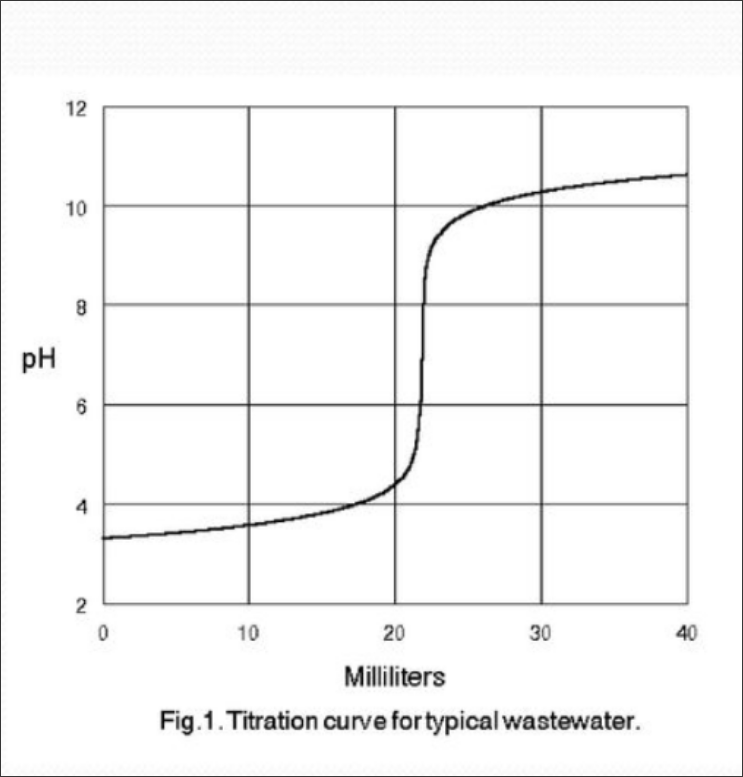
\includegraphics[width=15cm]{ph_curve.png}
		\end{figure}

		When using a pH logger, points beyond the equivalence point should be collected to make the inflexion more obvious

		Polyprotic acids (eg. \ce{H3PO4}) have multiple equivalence points, therefore will have three endpoints. Each "curve" represents the equivalence point of each of the three hydrogen ions

		\begin{figure}[H]
			\centering
			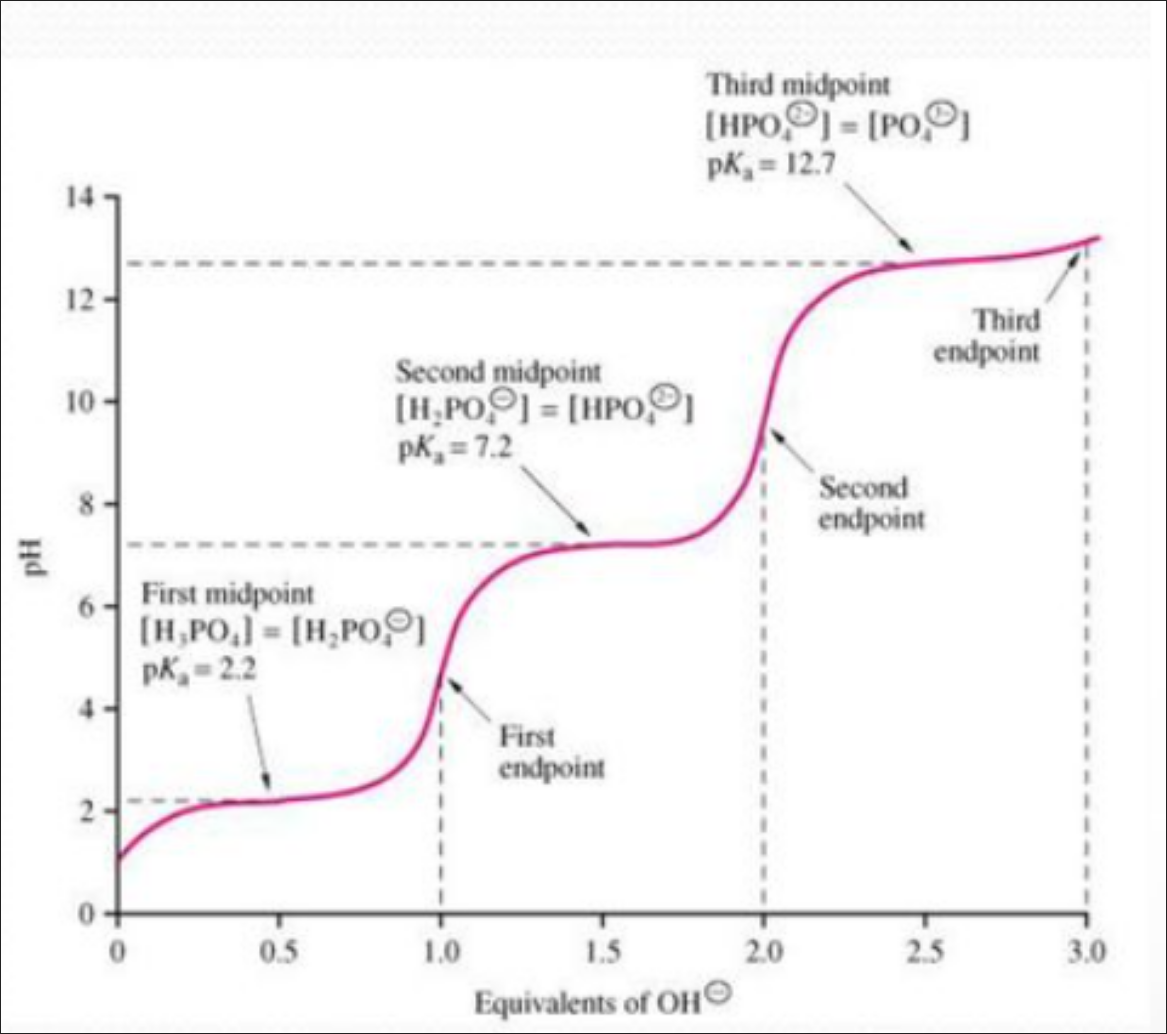
\includegraphics[width=15cm]{polyprotic_curve.png}
		\end{figure}

	\subsection{Activity Sheet 7.4 - Titration Curves}
	
		\subsubsection{Titration of the strong acid in solution}
		
			\begin{enumerate}
				\item What would you expect to be the pH of the titration solution after exact neutralisation of a strong acid with a strong base? If an indicator that changes colour close to this pH were used, would the colour change indicate the equivalence point accurately?
					The pH would be around a pH of 7. If an indicator was used, the pH could be accurately determined through a colour change.

				\item Suppose that we use an indicator that changes colour near pH 5. According to the graph, does the colour change endpoint accurately indicate the equivalence point? Explain why this is the case.

					The equivalence point determined by the graph is around 10. Therefore, an indicator that demonstrates a colour change near a pH of 5 would not be appropriate.

				\item If we use an indicator that changes colour near pH 9, does the colour change endpoint accurately indicate the equivalence point? Explain why.

					Yes. The equivalence point sits around pH 9, therefore an indicator around this would be appropriate.

			\end{enumerate}
		
		\subsubsection{Titration of the weak acid in solution}

			\begin{enumerate}
				\item If a solution of a weak acid is titrated with a NaOH solution, would you expect the pH at exact equivalence to be at pH = 7, at pH $>$ 7, or at pH $<$ 7? Explain why.
					
					\ce{NaOH} is a strong base, therefore when combined with a weak acid the resulting solution would be basic, ie. pH $>$ 7.

				\item Suppose we use an indicator that changes colour near pH 9. Reading the graph as accurately as possible, what volume of titrant (the NaOH solution) is added before the indicator changes colour? Does the indicator colour-change endpoint accurately indicate the equivalence point?
			\end{enumerate}


\section{Acid/base Analysis by Aboriginal and Torres Strait Islander Peoples} \label{20/03/2025}

	\subsection{Grey Mangroves}
	
		The grey mangroves are  used to treat stingray injury by prevent infection and neutralise the mildly acidic stingray venom. This is done by smashing the grey mangroves' leaves to create a basic mixture that can be applied to the wound caused by the stingray

	\subsection{Yellow Ochre}
	
		Aboriginal and Torres Strait Islander Peoples used yell ochre (hydrated iron hydroxide) to treat stomach upsets. The yellow ochre is basic and can react and neutralise with any excess hydrochloric acid in the stomach

	\subsection{Davidson Plum}
	
		The Davidson plum is a natural Australian fruit with 100 times more of ascorbic acid (vitamin C) than contained in an orange. Therefore, it is very sour

		Aboriginal and Torres Strait Islander Peoples consumed the Davidson plum as way to boost their body’s nutrient level which reduced their chance of having scurvy disease.

	\subsection{Soap Tree}
	
		Soap tree's leaves contain saponin acid that has the ability to suppress bateria growth

	\subsection{Goat's Foot (Coastal Morning Glory)}
	
		The leaves (heated on rocks) can be applied as a poultice were used to relieve stings and bites from insects. It is poisonous if incorrectly applied

	\subsection{Clay Eating}
	
		Clay possesses antacid and ati-diarrhoeal functions by assisting with the absorption and assimilation of fluids into the intestine, in which it acts to prevent fluid loss through diarrhoea.

		Clay has the ability to deactivate toxins within the stomach. This increases the tolerance of poisonous plants and unlock a forbidden diet

		It acts as a detoxifying agent. This property is referred to as its poly cationic nature, which leads to the absorption of negative charge toxins. It works like activated charcoal which is known as a digestive aid.

		Its magnetic feature draws cadium, lead, and other toxins to it. The clay moves the toxins molecules through the intestines

\section{Conductometric Titration}

	Another method of determining when the equivalence point is reached is by \textbf{measuring the change in conductivity of the analyte using a conductivity probe}. Conductivity refers to a flow of ions that can be positive or negative, ie. not necessarily electricity. A titration that uses this property is called a conductometric titration.

	\subsection{Advantages}
	
		Can be applied to:
		\begin{itemize}
			\item Very diluted solutions - species at trace levels
			\item Coloured or turbid solutions
			\item Relatively incomplete reactions
			\item Acid-base, redox, precipitation and non-aqueous titrations
		\end{itemize}

	\begin{itemize}
		\item The electrical conductivity of a solution depends on the concentration of ions in the solution
		\item Conductivity of strong base or strong acid is stronger than that of a weak base or weak acid
		\item Change in conductivity during conductometric titration is due to one of the ions being replaced by another of different conductivity
	\end{itemize}

	Equivalence occurs when conductance is at minimum - no free ions. It does not reach 0 because there are still some ions present to transfer charge

	\textbf{Example Question (HSC 2019 Q24)}
	
	The graph initially shows a negative gradient as barium hydroxide solution is introduced into the standardised \ce{HCl} solution. This is due to the reaction of \ce{H+} ions in the \ce{HCl} solution with the \ce{OH-} ions from the barium hydroxide. This decreases the number of conductive ions in the solution, hence decreasing the solution's conductivity. When the equivalence point is reached (around 17mL), the number of \ce{OH-} ions present exceed that of \ce{HCl}, therefore the number of \ce{OH-} ions increases and the graph depicts the solution has an increase in conductivity.

	\textbf{Example Question (HSC 2024 Q34)}
	
	\begin{center}
		\ce{H+(aq) + NH3(aq) -> NH4+(aq)} \\
		\ce{NH3(aq) + HCl(aq) <=> NH4Cl}
	\end{center}

	The graph initially decreases in conductivity as ammonia solution is introduced. This is due to hydrochloric acid being neutralised by the added ammonia.

	The highly conductive \ce{H+} ions react with the \ce{NH3} ions, decreasing the overall conductivity of the solution.

	After the equivalence point, the excess ammonia will produce some \ce{NH4} and \ce{OH-} ions, both of which have greater conductivity than the reactant molecules.

\section{Back Titration} \label{21/03/2025}

	Back titrations are indirect titrations that can be used when:

	\begin{itemize}
		\item the reaction is too slow so it is difficult to determine endpoints
		\item the sample is not soluble in water, but will react with an acid for example
		\item the sample is toxic
		\item the sample is volatile
		\item the sample is gaseous and in a mixture of gases
		\item the sample is fairly unreactive
	\end{itemize}

	\textbf{Example}
	
	A back titration could be used to determine the percentage of calcium carbonate in a sample of limestone. It is not soluble in water, so it cannot be dissolved to form a solution. However, it will react with \ce{HCl}. For example:

	\begin{center}
		\ce{CaCO3(s) + 2HCl(aq) -> CaCl2(aq) + CO2(g) + H2O(l)}
	\end{center}

	A known excess volume of a standardised \ce{HCl} solution (this can be created by titration) would be added to the limestone. It is assumed that the acid only reacts with calcium carbonate, not with any of the other impurities. If the \ce{HCl} reacts with impurities, the final result will be greater than the actual amount of \ce{CaCO3} present.

	The least amount of measurements made reduces the amount of total errors in the experiment and providing a more accurate result.

\section{Titration of Household Chemicals} \label{27/03/2025}

	\subsection{Wine Industry}
		
		The use of analytical instruments in the wine industry allows scientists to learn more about the

		As fermentation proceeds, the density of the mixture decreases. This is due to ethanol's lower density in comparison to water.
	
		Titration to find \ce{SO2} content in wine
		
		Sulphur dioxide is used to kill or inhibit unwanted yeasts and bacteria in wine and to protect the wine from oxidation. When sulphur dioxide is added to wine, there are three forms present: molecular \ce{SO2}, \ce{SO3^{2-}} and smth

	\subsection{Mining Industry}
	
		Ore needs to be dissolved to be tritrated. Done using particular acids. 

\newpage

\section{Buffers} \label{07/04/2025}
	
	\textbf{Keeping the balance}
	
		It is important that environments meet the needs of the organisms that live there. This means that conditions such as pH, concentration of ions, and temperature are maintained at suitable levels.

		In a natural environment, the levels of these conditions in a particular environment will dictate what organisms are able to survive
	
	\subsection{Buffers}
	
		Buffers are utilised in the natural environment and biological systems to maintain an optimal pH.

		It is a solution of a weak acid and its conjugate base (or vice versa) that is \textbf{able to resist a change in pH} when an acid or base is added

		It achieves this due to the equilibrium established between the weak acid (or base) and its conjugate.

		\textbf{Example}
		
		A solution of carbonic acid and sodium hydrogen carbonate (\ce{H2CO3} / \ce{HCO3-})

		The pH of a buffer is determined by the:

		\begin{itemize}
			\item Equilibrium constant $K_a$ of the weak acid
			\item Ratio of weak base [\ce{A-}] to weak acid {\ce{HA}} in solution
		\end{itemize}

		If a buffer has more acid than base, more \ce{H+} ions are present and the pH is lower.

		When the concentrations of \ce{A-} and \ce{HA} are equal, [\ce{H+}] is equal to $K_a$ and the pH is equal to pKa.

		\begin{center}
			\ce{HA(aq) + H2O(l) <=> A-(aq) + H3O+(aq)}
		\end{center}

		When a strong acid is added, LCP pushes the reaction to the left. The pH will increase near to the original value.

		When a strong base is added, the concentration of \ce{H3O} decreases and the system will oppose this change. The pH is decreased to near the original value.

		The pH is maintained by manipulating the proportion of weak base (\ce{A-}) and weak acid (\ce{HA}) in solution. As long as $\frac{[\ce{A-}]}{[\ce{HA}]}$ is between 0.1 and 10, the pH is within 1 unit and the solution is therefore buffered.

	\subsection{Buffer Capacity}
	
		The buffer capacity is the amount of the acid or base that can be added without a significant change in pH. The buffer capacity is greatest when there are equal number of moles of the weak acid and the conjugate base. In this case, it can counteract both the addition of an acid or base. The more of each weak acid and conjugate base, the greater the buffer capacity.

	\subsection{Buffering in the Environment}
	
		With increasing carbon dioxide levels in the atmosphere, there is a major concern that the oceans and soil are being acidified.

		In ocean waters, carbon dioxide is found in higher concentrations than other non-polar gases as it reacts with water. The changes in pH at these levels are significant and are altering the thickness of shells of aquatic organisms and the ability of organisms to take up calcium.

	\subsection{Buffer in sea water}
	
		In sea water, the buffer is due to bicarbonate and carbonate ions.

		In the following reaction:

		\begin{center}
			\ce{HCO3-(aq) + H2O(l) <=> CO3^{2-}(aq) + H3O+(aq)}
		\end{center}

		The \ce{HCO3} is the weak acid, and \ce{CO3^{2-}} is its conjugate base.

		With increasing carbon dioxide levels in the atmosphere, there is a major concern that the oceans are being acidified. The breakdown of organic matter and fish waste also causes the water to become more acidic. The buffer is able to counteract this change so that the pH is not affected.

		Calcium and magnesium ions cause the water to become more alkaline. This happens when items such as shells are added to the environment and when minerals in the surrounding soil are in run-off entering the water.

		Natural sea water has a pH of 8.0 - 8.3. At this pH, there are appropriately equal amounts of bicarbonate and carbonate ions.

	% !TEX root = ./chemistry.tex

\chapter{Module 7 - Organic Chemistry}

\section{Hydrocarbons} \label{02/05/2025}

	\subsection{Bonding in Carbon}
	
		Carbon atoms almost always form four covalent ($\because$ non-metal) bonds because of it's valency of 4.

		In alkanes (single bond compounds)

		One, two or three pairs of the valence electrons from adjoining carbon atoms may be involved in the bonding to form :

			\begin{itemize}
				\item single bonds \ce{C-C}
				\item double bonds \ce{C=C}
				\item triple bonds \ce{C#C}
			\end{itemize}

		When four carbon atoms bond to each other, a different type of substance forms. This is due to the varying structures in each type of covalent network lattice. Each structure is called an \textbf{allotrope}

	\begin{figure}[H]
		\centering
		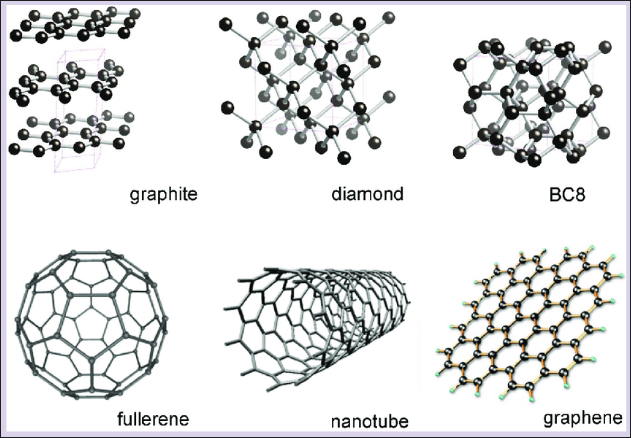
\includegraphics[width=8cm]{covalent_carbon_structure.png}
	\end{figure}

	\subsection{Types of Hydrocarbons}
	
		Hydrocarbons are compounds made up of only hydrogen and carbon

		\textbf{Aromatic} hydrocarbons contain one or more benzene rings

		\textbf{Aliphatic} compounds are all the other hydrocarbons. The carbon atoms may be bonded in chains or non-aromatic rings. The chain of compounds may be further classified into families on the basis of individual carbon-carbon bonds.

	
	\subsection{Aliphatic Hydrocarbons}
	
		\begin{enumerate}
			\item If all carbon-carbon bonds are single bonds, the compound is an \textbf{alkane}. These are called \textbf{saturated compounds}.
			\item Compounds in which at least one of the carbon-carbon bonds is a double bond are called \textbf{alkenes}. Compounds with at least one multiple bond are called \textbf{unsaturated compounds}.
			\item Alkynes have at least one carbon-carbon triple bond. They are classified as unsaturated compounds.
			\item Hydrocarbon compounds in which the carbon atoms have joined to form a closed ring structure are called \textbf{alicyclic}, or more commonly, cyclic hydrocarbons.
		\end{enumerate}

	\subsection{Representing Organic Molecules}
	
		A \textbf{molecular formula} such as \ce{C3H8} gives information on the number of atoms, but nothing about the arrangement of those atoms.

\textbf{Structural formulae} are used to represent organic molecules as the arrangement of atoms can vary greatly within molecules with the same molecular formula.

	\subsection{Check Your Understanding - 8.1}
	
		\begin{enumerate}
			\item \textbf{Describe how the valence electrons of carbon are involved in bonding in organic compounds}
				\subitem The four valence electrons in the carbon atom allow it to form four covalent bonds with other atoms

			\item \textbf{Describe the differences between:}
				\begin{enumerate}
					\item aromatic and aliphatic compounds - aromatic compounds contain a benzene ring whereas aliphatic do not
					\item saturated and unsaturated compounds - saturated only single, unsaturated have varying
				\end{enumerate}
		\end{enumerate}

\section{Alkanes}

	Alkanes are important because it includes the fuels that supply energy

	Light gases have small molecules with:

	\begin{itemize}
		\item Low boiling point
		\item Light in colour
		\item Easy to light
		\item Runny
	\end{itemize}

	Including methane, ethane, propane, and butane

	Longer chained hydrocarbons have a higher boiling point. When boiling, intermolecular forces are broken (which are dispersion forces in hydrocarbons). The longer the chains, the more hydrogen is present, making it harder to separate each molecule apart.

		\subitem 1 - meth

		\subitem 2 - eth

		\subitem 3 - prop

		\subitem 4 - but

		\subitem 5 - pent

		\subitem 6 - hex

		\subitem 7 - hept
		
		\subitem 8 - oct
		
		\subitem 9 - non

		\subitem 10 - dec

	The alkanes are known as a homologous series; a group of compounds with the same general formula.
	
	\subsection{Rules for Naming Alkanes}
	
		\begin{enumerate}
			\item The end of the name indicates which hydrocarbon family the compound belongs in. Alkanes end in -ane.
			\item Determine the longest continuous carbon chain and use the name of the corresponding alkane. This is the \textbf{main chain}.
			\item Other atoms of groups of atoms attached to the main chain are called substituents and form "branches". If the substituent is a carbon group, then it is called an alkyl group. Alkyl groups are given the ending -yl.
			\item Number the carbons in the main chain so the branch of branches have the lowest possible numbers.
			\item The position at which the group is attached to the main chain is specified by the number of the carbon to which it is attached. The number is separated by a hyphen.
			\item The names of the substituents are given in \textbf{alphabetical order}.
		\end{enumerate}

\section{Alkenes} \label{07/05/2025}
	
	The alkene family contains hydrocarbons in which one pair of carbon atoms is joined by a double bond, and all other carbons are joined by single bonds. This double bond means that the hydrocarbon is unsaturated.

	Alkenes have the general formula \ce{C_{n}H_{2n}}

	\subsection{Naming Alkenes}

		The process of naming alkenes is similar to that of alkanes, however the position of the double bond can change.

		\begin{enumerate}
			\item Take the usual stem name (eg. eth-, bu-) and add the suffix -ene.
			\item Show the location of the double bond by numbering the carbon atoms from the end of the chain closest to the double bond; ie. get the smallest number, eg. a 1-butene hydrocarbon would have a double bond between the 1 and 2 carbon atoms
			\item Branched alkenes have the same rules as branched alkanes
			\item The double bond is prioritised over substituents when determining the end of the hydrocarbon to start at
		\end{enumerate}

\section{Alkynes} \label{08/05/2025}

	Alkynes are a family of hydrocarbons containing at least one triple bond between a pair of carbon atoms. Like the alkenes, alkynes are unsaturated.

	Alkynes have a general form of \ce{C_{n}H_{2n-2}}

	The naming process is identical to that of alkenes

\section{Halogenated Organic Compounds}

	Organic compounds that contain one of more halogen atoms (bromine, chlorine, fluorine, or iodine) attached to one of the carbon atoms in the molecule.

	\subsection{Naming Hydrocarbons with Halogen Atoms}
	
		\begin{enumerate}
			\item Name the parent chain as normal
			\item Alkyl side chains are identified and named as normal
			\item Any halogen atoms are identified with the place number of the carbon they are attached to. Their name is given as follows:
				\begin{itemize}
					\item fluorine $\rightarrow$ -fluoro
					\item chlorine $\rightarrow$ -chloro
					\item bromine $\rightarrow$ -bromo
					\item iodine $\rightarrow$ -iodo
				\end{itemize}
			\item All branches are listed in alphabetical order
		\end{enumerate}

\section{Isomers}

	Compounds that have the same molecular formula but different structural formula are called structural isomers.

	In hydrocarbons, isomers can occur by changing the position of double or triple bonds, or different placement of substituents (positional isomers).

	Chain isomers involve rearrangement of the carbon skeleton.

\section{Benzene}

	An unsaturated aromatic compound with delocalised electrons with formula \ce{C6H6}. It has a shape of a flat hexagon

	Benzene rings have carbon bonds of the same length, however the length of the each bond lies between a single bond and a double bond. The double bonds are not drawn because they can exist either in place 1, 3, 5 or 2, 4, 6 with each structure being structurally equivalent. A circle is drawn in the centre to represent the electron cloud.
	
	\begin{center}
		\chemfig{C*6((-H)-C(-H)=C(-H)-C(-H)=C(-H)-C(-H)=)}
	\end{center}

	The cyclic delocalisation of electron makes it extremely stable

\section{Properties of Alkanes}

	Alkanes are covalent molecular substances so they will have similar physical properties to other covalent molecules.

	Carbon and hydrogen have similar electronegativity and most hydrocarbons are relatively symmetrical, making them non-polar.

	Alkenes and alkynes have a similar structure to alkanes, and so share the same physical properties.

	Alkanes have relatively low melting and boiling points since dispersion forces are the only type of intermolecular force that forms between molecules. As the size of the molecule increases, more atoms are present, increasing the number of electrons in the molecule. Thus the strength of the overall dispersion forces between molecules increases.

	Larger molecules require more energy to overcome the dispersion forces, hence \textbf{Longer carbon changes have higher melting and boiling points}

	For example, shorter chain alkanes like ethane and propane are gases at room temperature in comparison to octane and oils being liquids and very long chains like wax and tar being solids.

	The shape of the hydrocarbon also changes the boiling and melting points of a compound. Linear molecules pack closely and allow many dispersion forces to form, creating a greater attraction between molecules. Bulky molecules no not neatly pack together, therefore have smaller boiling and melting points.

	Lack of polarity means that hydrocarbons are not conductive or soluble in water

\section{Uses of Alkanes}

	\begin{itemize}
		\item Methane is a main component of natural gas
		\item Propane is also known as liquid petroleum gas (LPG)
		\item Pentane is used as an industrial solvent
		\item Octane is the main constituent of automobile fuel
		\item Nonane and decane are used in petrol as additives
	\end{itemize}

\section{Uses of Alkenes}

	\begin{itemize}
		\item Basis of petrochemical industry, especially those with low molecular mass
		\item Used as starting materials in the syntheses of alcohols, plastics, lacquers, detergents, and fuels
		\item Ethene is the most important organic feedstock in the chemical industry. A feedstock is a chemical or substance that is used to manufacture useful materials and other chemicals
		\item Used for making polyethylene, vinyl chloride, styene, artificial ripening of fruits, general anaesthetic
	\end{itemize}

\section{Functional Groups}

	A group or family of organic properties. Substances within a particular family containt a specific atom or group of atoms called a functional group.

	\begin{table}[H]
		\centering
		\setstretch{1.25}
		\begin{tabular}{l|l|l}
			Class & Suffix & Functional Group \\ \hline
			Haloalkane & -ane & -F, -C, -Br, -I \\
			Alcohol & -ol & -OH \\
			Aldehyde & -al & -C=O,-H \\
			Ketone & -one & \\
			Carboxylic acid & -oic acid & \\
			Ester & alkyl -oate & \\
			Amine & -amine & \\
			Amide & -amide &
		\end{tabular}
	\end{table}

\section{Alcohols}


	\subsection{Naming Alcohols}
	
		\begin{enumerate}
			\item Identify the longest carbon chain
			\item Write the alkane name without the "e" at the end and replace it with "ol"
			\item Similar to identifying the position of the double bond in alkenes, the position of the \ce{-OH} group is identified by using a number in front of the main alcohol name
		\end{enumerate}

	\subsection{Types of Alcohols}
		
		Alcohols can be classified according to the number of carbon atoms attached to the carbon bearing the \ce{-OH} group.

		Primary: butan-1-ol

		\begin{center}
			\chemfig{CH_3-CH_2-CH_2-CH_2-OH}
		\end{center}

		Secondary: butan-2-ol

		\begin{center}
			\chemfig{CH_3-CH_2(-[2]CH_3)-CH_2-CH_3}
		\end{center}

	\subsection{Properties of Alcohols}
	
		The hydroxyl group in alcohols contains a highly electronegative oxygen atom, thus making a highly polar \ce{C-O} and \ce{O-H} bond.

		The properties of alcohols depend on the presence of the \ce{-OH} group and the size of teh hydrocarbon chain.

		The boiling point of an organic compound relates to the energy required to overcome intermolecular forces between molecules.

		Hydrogen bonding in alcohols is stronger than dispersion forces, therefore it will have a significantly higher boiling point than alkanes of similar molecular mass.

	\subsection{Solubility}
	
		Alcohols with a smaller hydrocarbon chain are very soluble in water. The polar \ce{-OH} group forms hydrogen bonds with water, making short chains soluble. The non-polar hydrocarbon chain cannot form hydrogen bonds so is not soluble. As the length of the hydrocarbon chain increases, the solubility decreases.

		An example of a large molecule with high solubility in water is glucose, \ce{C6H12O6}

\section{Aldehydes and Ketones} \label{12/05/2025}

	Carbonyl compounds are those double bonded to an oxygen atom. Both aldehyde and ketones are carbonyl compounds.

	Aldehydes are carbon compounds that contain a carbon-oxygen double bond at the end of the carbon chain. The compound is represented by the general molecular formula:

	\begin{center}
		\chemfig{R-{CH}(=[2]O)}
	\end{center}

	Methanal (\ce{HHCO}), commonly known as formaldehyde is the simplest aldehyde. Methanal is used in vast quantities in the manufacture of plastics.

	Ketones differ from aldehydes in that the \ce{C=O} can be located on any carbon except those at the ends of the hydrocarbon chain. The compounds have the general formula:

	\begin{center}
		\chemfig{R-C(=[2]O)-R'}
	\end{center}

	Propanone is widely used as a solvent, and is commonly known as acetone

	\subsection{Functional Group Isomers}
	
		Aldehydes and ketones are known as functional group isomers. These have the same molecular formula but different structures.

	\subsection{Properties of Aldehydes and Ketones}
	
		Oxygen is more electronegative than carbon, so it has a high tendency to attract electrons in the carbon-oxygen bond and is therefore highly polar. This polarity allows dipole-dipole forces to interact.

		As a result, aldehydes and ketones have higher boiling points than hydrocarbons of similar mass. Alcohols form stronger hydrogen bonds and have higher boiling points.

		The carbonyl group, being highly polar, does form an attraction to highly polar water molecules. This makes aldehydes and ketones more soluble than hydrocarbons but less soluble than alcohols.

		Small aldehydes and ketones are soluble in water, but as the chain length increases, solubility in water decreases.

		\subsubsection{Examples}
	
			Select the compound in each pair that would have the higher boiling point.

\section{Carboxylic Acids}

	Includes acetic acid, butanoic acid, citric acid. Many of them have strong and unpleasant odours.

	Carboxylic acids contain the carboxyl functional group, which is always found at the end of the parent chain of the molecule.

	Many carboxylic acids have common names.
	\begin{itemize}
		\item Methanoic acid is formic acid
		\item Ethanoic acid is more commonly known as acetic acid
		\item Propanoic acid is also propionic acid
	\end{itemize}

	\subsection{Naming Carboxylic Acids}
		
		\begin{enumerate}
			\item Add "oic acid"
			\item Number the carbon atoms from the main chain. Like aldehydes, no number is needed because it is at the start
		\end{enumerate}

	\subsection{Properties of Carboxylic Acids}
		
		The presence of the \ce{OH} and \ce{C=O} groups makes the entire carboxyl group polar. THey are capable of forming a range of intermolecular forces.

		Since it requires more energy to overcome the intermolecular forces between carboxylic acid molecules, this group will have higher boiling points than other molecules of similar size

		Under certain circumstances, a pure carboxylic acid will form a structure called a dimer.
		
		Small carboxylic acids are very soluble in water due to hydrogen bonding with water. In smaller acids, the effect of the non-polar hydrocarbon chain is outweighed by the effect of the highly polar carboxyl groups.

		In longer chains, the hydrophilic heads are at the water surface (surfactants) whereas the "tails" (the non-polar chain) do not mix with water.

	\subsection{Monoprotic Nature}
	
		The carboxylic acid group is monoprotic. This is because the only H atom that can react with a base is the one in the \ce{-COOH} group.

		Carboxylic acids are weak acids, so they will partially ionise in solution, producing hydrogen ions. Different acids ionise to different extents.

		The strength of a carboxylic acid can be increased by substituting a highly electronegative atom such as a halogen onto the hydrocarbon chain. As the number of substituted atoms increases, so does the strength of the acid. This is because the strong electron-attracting power of the substituent weakens the oxygen-hydrogen bond in the \ce{-OH} group and makes it easier to form \ce{H+} bonds.

\section{Amines and Amides}

	Amines have a wide range of uses as catalysts and solvents and in the manufacture of dyes, medicines and polymers, so they are an extremely important family of organic compounds. Amines are also widely found in nature as amino acids, which are the building blocks of proteins.

	An amide is formed when an amine reacts with a carboxylic acid. Polyamides are an important group of synthetic plastics.

	Urea, an important compound in industry and living systems, is also known as carbamide with the formula \ce{H2N-CO-NH2}. It has two \ce{NH2} groups attached to a carbonyl (\ce{C=O}) group. Urea was the first organic compound to be synthesised from inorganic starting materials, thus showing organic compounds were part of a chemical system and could be produced outside living things.

	The amine or amino functional group is \ce{-NH2}. Amines are compounds in which one or more atoms of hydrogen in ammonia are replaced by a carbon-containing group, such as an alkyl group. Alkyl amines are represented by the general formula \ce{RNH2}.

	\begin{center}
		\chemfig{{CH3}-{CH}(-[6]{CH3})-{CH}(-[6]{NH2})-{CH3}}
	\end{center}

	\subsection{Properties of Amines}
	
		Nitrogen is the third most electronegative element, so the \ce{-NH2} functional group is very polar. Nitrogen is less electronegative than oxygen, the hydrogen bonds formed by amines are weaker than those formed by alcohols. This results in the boiling points of amines being lower than those of similarly sized alcohols.

		The hydrogen bonding also means the smaller amines are soluble in water. Tertiary amines cannot form hydrogen bonds because there is no \ce{N-H} bond in the molecule. Consequently, their boiling points are lower than those of primary and secondary amines and are generally insoluble in water.

	
		Amides are the derivatives of carboxylic acids and are formed when the \ce{-OH} group of the acid is replaced by an amine (\ce{NH2}, \ce{NHR\'}) group.

	\subsection{Properties of Amides}
		
	Primary and secondary amides have two very polar bonds, the \ce{N-H} and the \ce{C=O}. Tertiary amides only have the \ce{C=O} since the nitrogen is attached to three alkyl groups, so no \ce{N-H} bond exists.

	This means primary and secondary amides can form hydrogen bonds between molecules. They can also form a dimer formation between the \ce{N-H} on one molecule and the \ce{C=O} of a different molecule.

\section{Hydrocarbon Reactions}

	\subsection{Using Organic Substances Safety}
	
		Safety precautions are managed using a Safety Data Sheet (SDS). All chemicals have an SDS that must be kept on the site where the chemical is used. Each SDS:

		\begin{itemize}
			\item details of the properties of a particular chemical
			\item identifies possible hazards and precautions for safe use and handling
			\item identifies steps to be taken to administer first aid upon contact, inhalation, or ingestion
		\end{itemize}

	\subsection{Hazardous Organic Compounds}
	
		\begin{itemize}
			\item Ethanal - used in polymer production -  toxic when inhaled, nervous system damage, pulmonary oedema
			\item Benzene - Production of plastics, resins, dyes - Toxic, is an anaesthetic
		\end{itemize}
	
	\subsection{Risks of Organic Chemicals}
	
	\subsection{Physical Properties}
		
			Many organic compounds are volatile. They have low boiling points and often evaporate at room temperature to form a vapour. The vapours are usually colourless, thus aren't easily seen however they almost all have pungent smells so can be detected.

			They are also highly flammable, especially when in the vapour form. This is related to \textbf{flashpoint}; the lowest temperature at which a liquid can form an ignitable mixture in air near the surface of the liquid. Flashpoints below 23 $\degree$C are considered as highly flammable compounds.

			Highly reactive, can react with air, water, or other nearby chemicals

			\subsubsection{Exposure method and effects}
			
				\begin{itemize}
					\item Inhalation into lungs
					\item Absorption through skin
					\item Ingestion
				\end{itemize}

			\subsubsection{Effects}
			
				Contact effects causes the solvent to dissolve fats in human skin and can remove the protective barrier. This allows chemicals to more easily enter the bloodstream

				Acute poisoning

				Chronic poisoning from continued exposure

			\subsubsection{Prevention}
			
				Many industries have moved to eliminate or substitute harmful chemicals. Isolation can also be used to protect people. Simple isolation includes use of a lab coat, safety glasses, and gloves to avoid possible contact and absorption through the skin

			\subsubsection{Disposal of organic compounds}
				
				The largest consideration when dealing with chemical waste is what can be washed down the sink and hat cannot. As a general rule, no organic waste should be washed down the sink, no matter how dilute. 

				There should always be a brown waste container when dealing with organic chemicals. During practical investigations, organic substances \textbf{should be used in very small amounts}.

\section{Unsaturated Hydrocarbon Reactions}

	Alkenes and alkynes are highly reactive due to the presence of the double or triple bond. They are weak and easier to break.

	Complete combustion of hydrocarbon produces carbon dioxide and water, as seen with pent-1-ene.

	One common addition reaction of both compounds is addition of hydrogen, in a reaction known as \textbf{hydrogenation}. Alkenes are converted to alkanes in this reaction, as seen with ethene forming ethane.

	This reaction will only occur in the presence of a metal catalyst because the reaction is slow.

	\begin{enumerate}
		\item The alkene molecule is absorbed onto the surface of the catalyst
		\item The hydrogen is absorbed onto the surface of the catalyst
		\item The hydrogen molecule is attached to the alkene
	\end{enumerate}

	Hydrogenation of alkenes is used to make margarine from edible liquid oils. Fats and oils are natural esters, both fats and oils contain long chain hydrocarbons. Fats are primarily saturated hydrocarbon chains whereas oils are unsaturated chains.

	Hydrogenation of alkynes requires a Lindlar catalyst (a heterogeneous catalyst consisting of palladium deposited on calcium carbonate). The catalyst acts as an inhibitor, preventing the alkene reacting further to an alkane.

	In a similar mechanism, halogen atoms like chlorine or bromine can be added across a double or triple bond. This is known as halogenation. Due to eh reactivity of halogens, a catalyst is not needed for this reaction to occur.

	Aqueous bromine (as opposed to liquid bromine) Bromine water is an oxidising, intense brown mixture containing diatomic bromine (\ce{Br2}) dissolved in water.

	For example in the reaction of propene and promine water, one bromine will attach to the propene, however a water molecule will usually attach to the second one forming an alcohol. Liquid bromine will generally form a alkane.

	Hydrogen halides are molecules with a hydrogen atom and a halogen atom like chlorine or bromine. Hydrogen chloride and hydrogen bromide are common hydrogen halides.

	To add water to an alkene, a dilute sulfuric acid catalyst is required. When water is added across a double bond, it forms an \ce{-OH} bond.

	The hydration of alkynes is catalysed by mercury(II) compounds and sulfuric acid. Addition of water to an alkyne will produce a ketone. The exception is hydration of ethyne that produces ethanal since a ketone cannot form with only two carbons in the chain.

	\subsection{Markovnikov's Rule}
		
	When an asymmetrical reagent (eg. \ce{H2O} or \ce{HBr}) is added to an asymmetrical alkene, there are two possible products, however one product predominates.

	The hydrogen adds to the end carbon since it has the greater number of hydrogens attached.

\section{Saturated Hydrocarbon Reactions}

	Combustion of alkanes is complete combustion when oxygen is present in excess:

		\begin{center}
			\ce{C3H8(g) + 5O2(g) -> 3CO2(g) + 4H2O(l)}
		\end{center}

	In many situations (furnaces and car engines), oxygen is not present in excess amounts. Under conditions of limited oxygen incomplete combustion occurs.

	The enthalpy of combustion values for each of the above reactions decrease as the levels of oxygen available decrease.

	Carbon monoxide impacts on human health at levels above 10 ppm. It binds to hemoglobins and prevents oxygen to join the cell so it can't be carried through the body.

	Soot are crystalline carbon particles that can coat the lung and impair respiration.

	In a substitution reaction, an atom of another element substitutes for a hydrogen atom. It only occurs with chlorine or bromine and need sufficient amounts of energy. This reaction will only occur if the mixture is subjected to UV light.

\section{Implications of Obtaining and Using Hydrocarbons}
	
	\subsection{Source}
	
		The primary source of hydrocarbons is from crude oil, a fossil fuel. 

		In Australia, some heavier fractions with 15-25 carbon atom chains undergo \textbf{catalytic cracking} to decompose them into smaller chains. The catalysts are zeolites (aluminosilicates), which are compounds containing aluminium, silicon, and oxygen. An example of a catalytic cracking reaction is:

		\begin{center}
			\ce{C15H32(l) -> 2C2H4(g) + C3H6(g) + C8H18(l)}
		\end{center}

		This is economical as the smaller chains have higher demand.

		Thermal cracking is also used to create more desirable products. High temperatures from 450-750 $\degree$C and pressures of 70 atmospheres are used to crack the hydrocarbons.

		Exxon Valdez oil spill in 1989 caused significant environmental damage in Alaska. Depletion of fish stocks, lasting effects on animal life.

		When incidents like this occur there is:

			\begin{itemize}
				\item Psychological stress (employment issues)
				\item Mortgage stress
				\item Legal action related to the compensation from the effects of the disaster
				\item Placing stress on welfare systems and the local communities to provide support for these people and their families
			\end{itemize}

	\subsection{Using Hydrocarbons}
		
		\subsubsection{The Greenhouse Effect}
		
			Carbon dioxide produced through the combustion of these fuels is a greenhouse gas, so it absorbs infrared radiation in the atmosphere. Carbon dioxide produced through fossil fuel combustion is a major contributor to the enhanced greenhouse effect.

			Carbon dioxide absorbs infrared radiation, so this increase in carbon dioxide means an increase in the amount of heat that is trapped in the atmosphere. The most obvious consequence of this additional heat is a rise in global temperature.

		\subsubsection{Consequences of Enhanced Greenhouse Effect}
		
			\begin{itemize}
				\item Glaciers in the Arctic and other areas have experienced shrinkage
				\item Land loss due to sea level rise
				\item Decrease in pH in the oceans (ocean acidification)
			\end{itemize}

			\begin{center}
				\ce{CO2(g) <=> CO2(aq)} \\
				\ce{CO2(aq) + H2O(l) <=> H2CO3(aq)} \\
				\ce{H2CO3(aq) + H2O(l) <=> H3O+(aq) + HCO3-(aq)}
			\end{center}
			
			CSIRO post combustion capture plants to investigate effectiveness. Normally in a coal-fired power station the gases are released. These can instead be passed through a carbon dioxide absorber to reduce the amount of carbon dioxide entering the atmosphere.

			Geosequestration is the process of storing carbon dioxide in the ground as an attempt to reduce the enhanced greenhouse gas effect.

\section{Alcohols}

	\subsection{Combustion of Alcohols}
	
		\textbf{Complete combustion} of ethanol releases approximately 1370kJ per mole of ethanol combusted, as per the reaction:

			\begin{center}
				\ce{C2H5OH(l) + 3O2(g) -> 2CO2(g) + 3H2O(l)}
			\end{center}

	\subsection{Enthalpy of Combustion of Alcohols}
	
		All combustion reactions are exothermic, releasing energy into the surroundings.

		The specific heat capacity ($c$) of a substance is the amount of heat required to increase the temperature of a unit mass of a substance by 1 degree celsius

		The change in enthalpy for a chemical reaction ($\Delta H$) is defined as the heat absorbed or released from a given reaction. The combustion reaction occurs with excess oxygen so there is no carbon left. The water produced is in liquid form for the enthalpy of combustion. The value for $\Delta H$ will always be negative (heat is released)

		\subsubsection{Measuring the Enthalpy of Combustion of Fuel}
		
			It is difficult to directly measure the heat released when a fuel undergoes combustion, so an indirect method is used by applying the LoCE. These experiments are calorimetric since they measure changes in temperature.

	\subsection{Practice}
	
		\textbf{A student measured 150 g of water into a flask and placed it above a spirit burner filled with ethanol. The temperature of the water initially was 19.1°C and the initial mass of the spirit burner and fuel was 160.25 g. The water was heated until the temperature reached 41.9°C. The spirit burner was reweighed and had a mass of 158.42 g. Calculate the enthalpy of combustion of the ethanol.}
		
		\begin{align*}
			\text{Mass fuel} = 160.25 - 158.42 &= 1.83g \\
			\Delta T &= 22.8
		\end{align*}

		\begin{align*}
			q &= mc \Delta T \\
			&= 150 \times 4.18 \times 22.8 \\
			&= 1.430 \times 10^4 J
		\end{align*}

		\begin{align*}
			M(\ce{C2H5OH}) &= (2 \times 12.01) + (6 \times 1.008) + 16.00 \\
				       &= 46.068 \text{ gmol}^{-1} \\
			\Delta H &= \frac{14.3}{0.0397} &= 360 \text{ kJmol}^{-1}
		\end{align*}

\section{Dehydration of Alcohols} \label{21/05/2025}

	Alcohols undergo dehydration reactions by losing water to form alkenes when heated with concentrated sulfuric or phosphoric acids. An alternative method of dehydrating alcohols involves passing gaseos ethanol over heated aluminium oxide powder. The aluminium oxide acts as a catalyst and cracks the ethanol into ethene and water vapour

	\begin{center}
		\ce{CH3-CH2-OH -> CH2=CH2 + H2O}
	\end{center}

\section{Substitution with Hydrogen Halides (HX)}

	When alcohols react with a hydrogen halide (HX), like hydrogen chloride or hydrogen bromide, a substitution reaction occurs. The products are an alkyl halide and water.

	\begin{center}
		\ce{R-OH + H-X -> R-X + H2O}
	\end{center}

	\subsection{Reactivity}
	
		In reactions with hydrogen halides, tertiary alcohols are most reactive and will have very fast reactions with \ce{HX}. Primary alcohols are the least reactive. Methanol is very difficult to react with \ce{HX}. Lower halogens are more reactive. Eg. \ce{HF} is very difficult to react due to its high electronegativity.

\section{Production of Alcohols}
	\begin{center}
		\ce{CH3CH2CH = CH2(g) + H2O(g) -> CH2CH3CHOHCH3(l)}
	\end{center}

	\begin{center}
		\ce{\chemfig{CH_3 - CH_2 - CH(-[6]Br) - CH3} + H2O -> \chemfig{CH_3 - CH_2 - CH(-[6]OH) - CH_2} + HBr}
	\end{center}

	Haloalkanes have carbon-halogen bonds that are easier to break than the \ce{C-C} or \ce{C-H} bonds.

	The \ce{C-F} bond is an exception to this, with a bond energy much higher than \ce{C-C} or \ce{C-H} bonds. They will not undergo reaction with water to produce alcohols.

	Reactivity to Produce Alcohols

	Tertiary haloalkanes are the most reactive, followed by secondary haloalkanes. Primary haloalkanes do react, however very slowly

	\subsection{Production from Fermentation}
	
		Fermentation is the process of converting simple sugars like glucose into ethanol in an anaerobic (no oxygen) environment. The balanced equation for this is:

		\begin{center}
			\ce{C6H12O6(aq) -> 2C2H5OH(aq) + 2CO2(g)}
		\end{center}

		Yeast in the absence of oxygen converts glucose to ethanol.

		Types of sugars:
		\begin{itemize}
			\item Glucose - Big ring structure hexagon
			\item Fructose - Same formula as glucose but in a pentagon
			\item Sucrose - Combination of glucose and fructose connected by shared oxygen with a missing \ce{H2O}
		\end{itemize}

		Glucose and fructose are monosaccharides (simple sugars). They both have the molecular formula \ce{C6H12O6} and are isomers. Monosaccharides have a single ring structure of either four, five, or six carbons

		Sucrose is a disaccharide consisting of two carbon rings. Two monosaccharides join in a condensation reaction to produce disaccharides and water. Most fruits that are used to produce alcohol contain a mixture of these three sugars. plus other sugars like galactose (isomer of glucose) and maltose (two glucoses).

		Polysaccharides join multiple rings to form a long chain. Many grains and vegetables are used to produce ethanol through fermentation. These contain either cellulose or starch, carbohydrates, also known as polysaccharides.

		Enzymes present in a fermentation can break down complex sugars into glucose, ie. breaking longer polymers into smaller chains.

	\subsection{Conditions for Fermentation}
	
		Must have a low temperature (eg. red wine cannot exceed 29$\degree$C)

		Yeast and enzymes involved are extremely temperature sensitive. Need appropriate porosity of yeast cell membrane.

		Also highly sensitive to pH. The ideal range is around 6.1-6.8 (slightly acidic), otherwise it will denature (break apart)

		Oxygen with oxidise the ethanal to produce ethanol and ethanoic acid. Therefore it makes wine taste like vinegar. THe liquid, usually water, allows the carbon dioxide produced to escape and not build up pressure inside the reaction vessel.

		The mixture must also be dilute, otherwise the ethanol would kill the yeast. Yeast will be killed when ethanol content reaches 14\% v/v. The ethanol can be distilled at the end of the process to remove excess water.

\section{Fuels from Different Sources}

	Fossil fuels are currently the primary source of fuel in society. Fossil fuels are produced over millions of years from decayed animal and plant matter. Coal, crude oil, and natural gas are all fossil fuels.

\section{Reactions of organic acids and bases}

	\subsection{Esters}

		Esters often have pleasant fruit odours and are responsible for the flavours and fragrances of many fruits and flowers.

		As well as being widespread in nature, esters are commonly used in industry. They can be synthesised easily and they are produced synthetically for use as artificial flavouring.

		\begin{center}
			\chemfig[angle increment = 30]{R -[1]C(=[3]O) -[-1]O -[1]R'}
		\end{center}

		This ester is found in pineapples, peaches, and apricots. The ester group formed is alos referred to as an ester link. The ester link joins teh alcohol and carboxylic acid that reacts to produce the ester. It has the suffix "oate"

		\subsubsection{Naming Esters}
		
			The first part of the name is the alkyl group directly attached to the oxygen of the ester group. Originally, this part of teh ester was the alcohol molecule it formed from. It is given the name in alkyl form; for example, one carbon is methyl, four carbons is butyl, six carbons is hexyl

			Carboxylic acids and esters are also functional group isomers. For example, the molecular formula of both propanoic acid and methyl ethanoate is \ce{C3H6O2}.

		\subsubsection{Properties of Esters}
		
			The presence of \ce{C-O} and \ce{C=O} make the ester group polar. However, esters tend to be liquids are room temperature with boiling points lower than carboxylic acid. This is because their main intermolecular forces are dipole-dipole forces taht are weaker than hydrogen bonding in carboxylic acids and alcohols.
			
			\begin{center}
				\chemfig[angle increment = 30]{R - C(=[2]O)(-[-2]O(- R'))}
			\end{center}

			No H-bond donors, only dipole-dipole forms. Esters are soluble in water

			Most esters are not very soluble in water due to the lack of hydrogen bonding and the presence of large hydrophoic alkyl groups. However, they are soluble in organic solvents.

		\subsubsection{Preparing Esters}
		
			Esters are produced by the reaction between an alcohol and a carboxylic acid. It is a condensation reaction.

			Ester formation is a very slow process. The rate of reaction can be increased by:

				\begin{itemize}
					\item Adding concentrated sulfuric acid to the reaction mixture, acting as a catalyst
					\item Heating to increase rate of reaction
				\end{itemize}

			Conventional heating of the mixture in an open container will evaporate the ester, therefore low temperature must be used.

		\subsubsection{Reflux}
		
			In ester formation, a process called reflux is used. Reflux is the process in which reactants are heated for an extended period of time without any loss of reactants or products. As the reaction mixture is heated, the volatile components evaporate and move into a vertical condenser where the gases are cooled so they return to the reaction mixture in the flask.

			The top must be opened so that gases do not build up pressure in the chamber. The water cooling around the neck will condense these gases and return them to the bottom of the flask.

			Boiling chips are used to avoid superheating. Superheating occurs when a liquid is heated above its boiling point without boiling. SUperheated solutions can flash boil, causing a sudden increase in pressure and often results in flask breakage.

			The sulfuric acid used to catalyse the reaction also acts as a dehydrating agent by removing water. Due to LCP, the yield of the final ester is increased.

		\subsubsection{Purifying an ester}
		
			Once reflux has been performed, the flask will contain a variety of organic and inorganic substances. Since it is an equilibrium reaction, there will be a mixture of both reactants and products, as well as the catalyst used

				\begin{itemize}
					\item Ester - not very soluble in water
					\item Carboxylic acid - soluble in water if small
					\item Alcohol - soluble if short chain
					\item Water - a product of the reaction and from any diluted solutions added
					\item Sulfuric acid - soluble in water
				\end{itemize}

				\begin{enumerate}
					\item Use a \textbf{separating funnel} to separate immiscible substances process. Immiscible liquids do not dissolve in each other and separate into two layers, with the denser layer on the bottom.
						\begin{itemize}
							\item Before using, wash with water to remove water soluble substances. The entire mixture from the reaction flask is poured into a separating funnel and water is added. After being left to stand, the mixture separates into two layers
							\item The organic layer contains the ester, and will be at the top of the funnel. This layer may also contain alcohol and carboxylic acid.
							\item To check the organic layer, water drops can be added to the solution. Water drops will pass through the organic layer and dissolve in the aqueous later.
						\end{itemize}
					\item Addition of sodium carbonate or sodium hydrogen carbonate will remove any carboxylic acid in a neutralisation reaction. Any water-insoluble carboxylic acid that is present will react with the carbonate ions to produce a water-soluble carboxylate ion (\ce{RCOO-})
						\begin{itemize}
							\item Water is added again to the separating funnel, and it will create another aqueous layer that can be discarded
						\end{itemize}
					\item \textbf{Distillation} must then be used to separate the alcohol to the ester. Due to the different boiling point of the ester, distillation can be used to isolate the ester.

				\end{enumerate}

	\subsection{Organic Acids}

		The most common organic acids are carboxylic acids. They are simple, straight chain carboxylic acids like methanoic and ethanoic acid, also also more complex acids like citric acid, fumaric acid, and malic acid

		Carboxylic acids react with active metals to produce a salt and form hydrogen gas. They also react with a base to produce a salt and water.

		\begin{center}
			\ce{CH3COOH(aq) + NaOH(aq) -> Na+(aq) + CH3COO-(aq) + H2O(l)} 
		\end{center}

	\subsection{Organic Bases}
		
		Amino acids - base and acid - are a natural molecule that contains both an organic acid and an organic base in the same molecule. There are 20 natural amino acids with only the R group changing between the different acids.

		\begin{center}
			\chemfig{H - N(-[6]H) - C(-[2]R)(-[6]H) - C(=[2]O) - OH}
		\end{center}

		Organic acids are generally weak acids in solution, so will only partially ionise when added to water. As a result of this they generally do not have very low pH values when in solution. Each organic acid ionises to a different degree, so for the same concentration different acids will have different pH values.

		Organic bases will react with acids to form a salt and water in a Bronsted-Lowry reaction. The reaction below shows the addition of \ce{HCl} to methananime to form methylammonium chloride:

		\begin{center}
			\ce{CH3NH2(aq) + HCl(aq) -> CH3NH3+Cl-(aq)}
		\end{center}

		Reaction iwth an acid forms a compounds called a \textbf{protonated amine} (conjugate acid of the amine)

	\subsection{Summarising Organic Compounds and Reactions}
	
\section{Analysis of Organic Substances} \label{28/05/2025}

	\subsection{Chemical Tests for Functional Groups}

		\begin{itemize}
			\item Carboxylic acid - Test with blue litmus paper, or react with sodium carbonate to produce bubbles (gas can be tested with lime water)
			\item Alkene - Add drops of bromine or bromine water to the organic solvent (the solution will go from orange brown to clear and colourless)
			\item Alcohol - Potassium permanganate (\ce{KMnO4}) will lose colour, however alkenes will also oxidise, add granules of calcium chloride to remove any water present, and then add a small piece of sodium that will produce hydrogen gas, add glacial (very concentrated) acetic acid and 2-3 drops of concentrated sulfuric acid.
		\end{itemize}
	
	\subsection{Alcohol Reaction with Sodium}
	
		Primary, secondary, and tertiary alcohols react with sodium, to form an alkoxide anion (\ce{RO-}) and hydrogen gas.

		\begin{center}
			\ce{2ROH + 2Na -> 2RO-NA+ + H2}
		\end{center}

		Sodium reacts vigorously with water, so any water must be removed by using granules of a dehydrating agent like calcium chloride. The production of gas is fastest for a primary alcohol.

	\subsection{Analytical Techniques: Faster and Better}
	
		\begin{itemize}
			\item Mass spectroscopy - high energy electrons
			\item Nuclear Magnetic Resonance (NMR) spectroscopy - radio waves
			\item Infrared spectroscopy - infrared waves
			\item UV-vis spectrophotometry - UV-visible waves
		\end{itemize}

		\subsubsection{Mass spectroscopy}

			This technique is usually used with gas chromatography before the process begins. A gas chromatograph will separate the unknown substances into pure substances.

			Mass spectroscopy can reveal the structure of a substance such as its molar mass and elements preset, and can detect isotopes of an element.

			An electron beam knocks off the electrons, positively charging it. It will also break bonds in the molecules.

			Graphs will show mass/charge ratio over abundance. It will only account for cations.

			The vacuum pump will remove ions with too large or too small mass/charge ratio.

			The most abundant peak is called the base peak and it is given a relative abundance of 100\%. The abundance of all other species is calculated in relation to this amount.

			The most important peak on the mass spectrum is the parent one because it gives the molecular mass of the sample.

			If only one element is being examined using mass spectroscopy, the different peaks will only be due to the presence of isotopes of that element. The position of the peaks indicates the relative isotopic mass and the height of the peaks indicates the relative abundance of each isotope.

		\subsubsection{Infrared spectroscopy}

			IR light source goes through the sample. The infrared light interacts with the sample and some of it is absorbed by the sample. The detector shows the gaps in the infrared wave.

			Infrared is a wave that is an oscillation in a medium of a particular frequency that carries energy.

			In polyatomic molecules such as water, bonds not only stretch, but also bend. The more energy that is provided, the more the bonds stretch and bend.

			In a symmetrical stretch, there is no net dipole and therefore cannot be seen by the infrared spectrogram (not infrared active). For carbon dioxide (\ce{O=C=O}), asymmetric stretching frequency occurs at 2350 cm$^{-1}$ and bending vibration occurs at 666 cm$^{-1}$.

			Diatomic molecules (eg. \ce{O2} and \ce{N3}) cannot be detected by infrared spectroscopy because no dipole is depicted.

			Heavier atoms require more energy to increase vibration. Double bonds require more energy than single bonds to increase vibration. Therefore, measurement of the absorbance will determine which bonds are present.

			During infrared spectroscopy, a sample is placed in a cell that is in a beam of infrared radiation. A number of different frequencies are absorbed by the compound.

			Not all of the infrared region is used, mid wavelength IR is used (between 400 to 4000cm$^{-1}$). The group frequency region between 4000 to 1450 cm$^{-1}$ is used to identify functional groups.

			The fingerprint region of a spectrum is useful for distinguishing between compounds with the same functional groups but not as useful as the higher wavenumber

			Useful peaks: (refer to slides on GC)

			\begin{itemize}
				\item broad, rounded peak, 3400-3200 cm$^{-1}$
				\item sharp, strong peak, 1850-1630 cm$^{-1}$
				\item Alkanes are below 3000, alkenes are above 3000 cm$^{-1}$
				\item triple bonds are very weak, around 2050-2250 cm$^{-1}$
			\end{itemize}

\section{NMR Spectroscopy} \label{02/06/2025}

	NMR stands for nuclear magnetic radiation spectroscopy. When matter is placed in a magnetic field, some nuclei act like microscopic magnetic compass needles.

	The charged nuclei spin and create small magnetic fields. Only nuclei with an odd number of nucleons (protons and neutrons) possess spin that creates the magnetic field. The most common nuclei studied are 1H and 13C. These nuclei are used to produce spectra. When in a magnetic field, the nuclei will align themselves with the field.

	Nuclei aligned with the field can absorb the energy of a radio wave and flip to a higher energy spin that isn't aligned when the radio waves have the exact frequency that matches the resonance of the nuclei.

	The nuclei in a higher energy state will flip back to the more stable energy state and release this energy in the process. The energy difference between these aligned and unaligned spins depends on the nature of the nuclei and its chemical environment.

	The energy required to flip the nucleus indicates the chemical environment of the nucleus. Only measures the environment that the hydrogens are in.

	\textbf{Example}
	
	For example, in ethane, each carbon atom is attached to another carbon as well as to three hydrogen atoms. Both the carbon atoms have the same chemical environment.

	\begin{center}
		\chemfig{C(-[2]H)(-[4]H)(-[6]H) - C(-[2]H)(-[0]H)(-[6]H)}
	\end{center}

	However, in aldehyde propanal, there are three different carbon environments and three different \ce{H} environments.

	\begin{center}
		\chemfig{C(-[2]H)(-[4]H)(-[6]H) - C(-[2]H)(-[-2]H) - C(=[1]O)(-[-1]H)}
	\end{center}

	Nuclei with lower electron density are less shielded and are more impacted by magnetic fields. Nuclei with high density are shielded, protecting the nucleus from the external magnetic field.

	\begin{align*}
		B_{\text{eff}} = B_o - B_{\ce{e-}}
	\end{align*}

	As the electron density increases, the frequency required to achieve resonance decreases. More shielded electrons will appear as low frequencies.

	Upfield and downfield describe low and high energy of signals respectively.
	
	NMR spectrometers use different magnetic fields and therefore have different resonant frequencies. The difference is divided by the absorption frequency of the reference, to produce a value called the chemical shift, $\delta$. This chemical shift is measured in parts per million is independent of the magnetic field, and hence, can be used for comparing spectra from any magnetic field.

	The most shielded compound is \ce{Si(CH3)4}, called tetramethylsilane (TMS). TMS is used as the zero and is the calibration peak generally shown on the right of every spectrum. Since every other compounds is less shielded than TMS, all other values appear on the left.

	The solvent used must have no magnetic dipole moment. Deuterium can be used instead of water to make the solvents \ce{D_2O} (10 protons, 10 neutrons), \ce{CD_2Cl_2} that are invisible to the NMR spectrometer.


	\textbf{High resolution NMR} gives more information, producing splits in the peak. The signal splitting shows the number of protons on adjacent atoms.

	\subsection{Spin-spin Splitting}
	
		The frequency difference, measured in Hz, between two peaks of the doublet is called the coupling constant, J.

		Two adjacent protons split an NMR signal into a triplet


\end{document}
